\subsubsection*{Figures ---}

Sur chaque figure, on superpose les KDE des densités de probabilité a posteriori obtenues à chaque \textit{run} (100 \textit{runs} au total) pour l'estimation de la position en $x$ et en $y$. Les valeurs réelles des coordonnées à retrouver sont en pointillés rouges.

\subsubsection*{Figures ---}

Sur chaque figure, on superpose les valeurs de $\tilde{\VecMu}_q$ estimée à chaque \textit{run} (100 \textit{runs} au total). La valeur réelle du débit est en pointillés rouges.
 
 
  \begin{figure}[p!]
  	\centering
  	\begin{subfigure}[t]{0.5\textwidth}
  		\centering
  		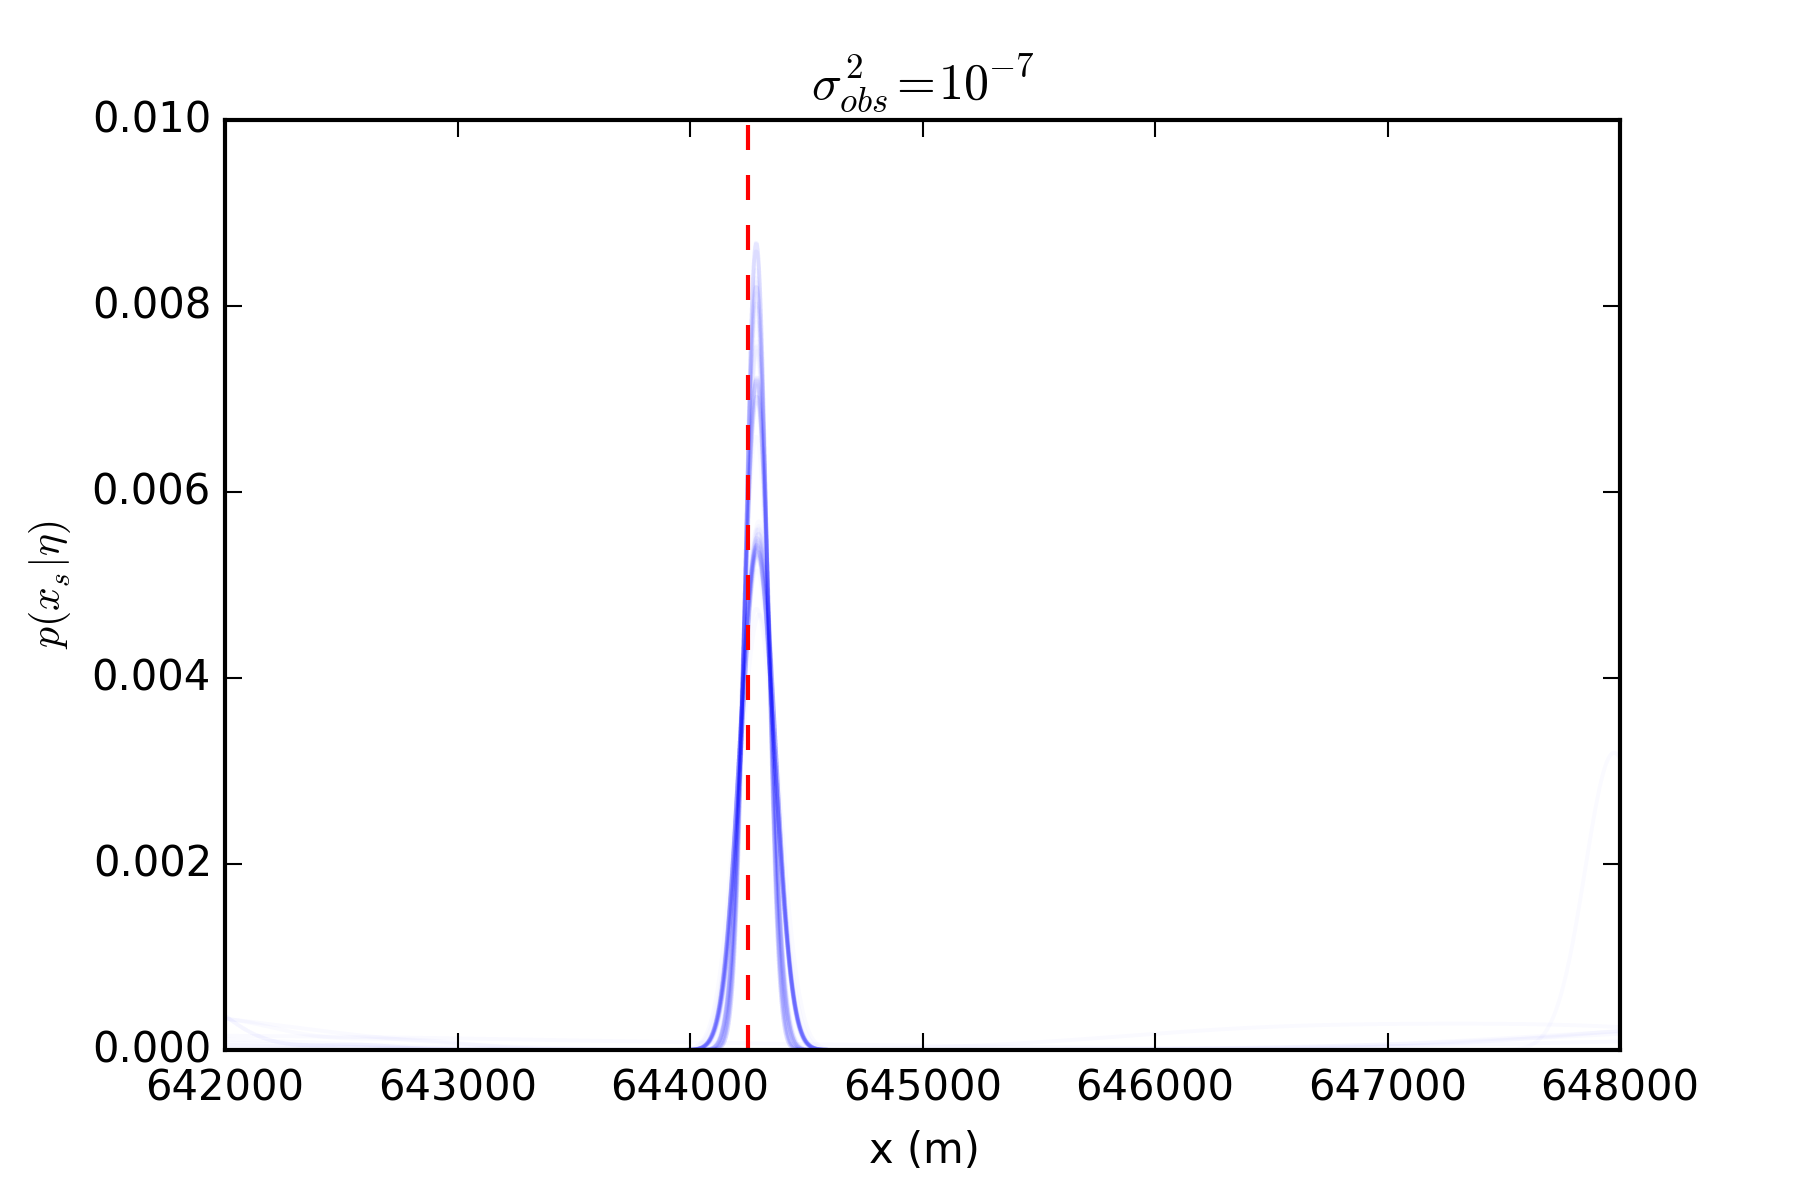
\includegraphics[width=1\textwidth]{25C_varobs_X_A.png}
  		\caption{}
  		\label{varA_x}
  	\end{subfigure}%
  	\begin{subfigure}[t]{0.5\textwidth}
  		\centering
  		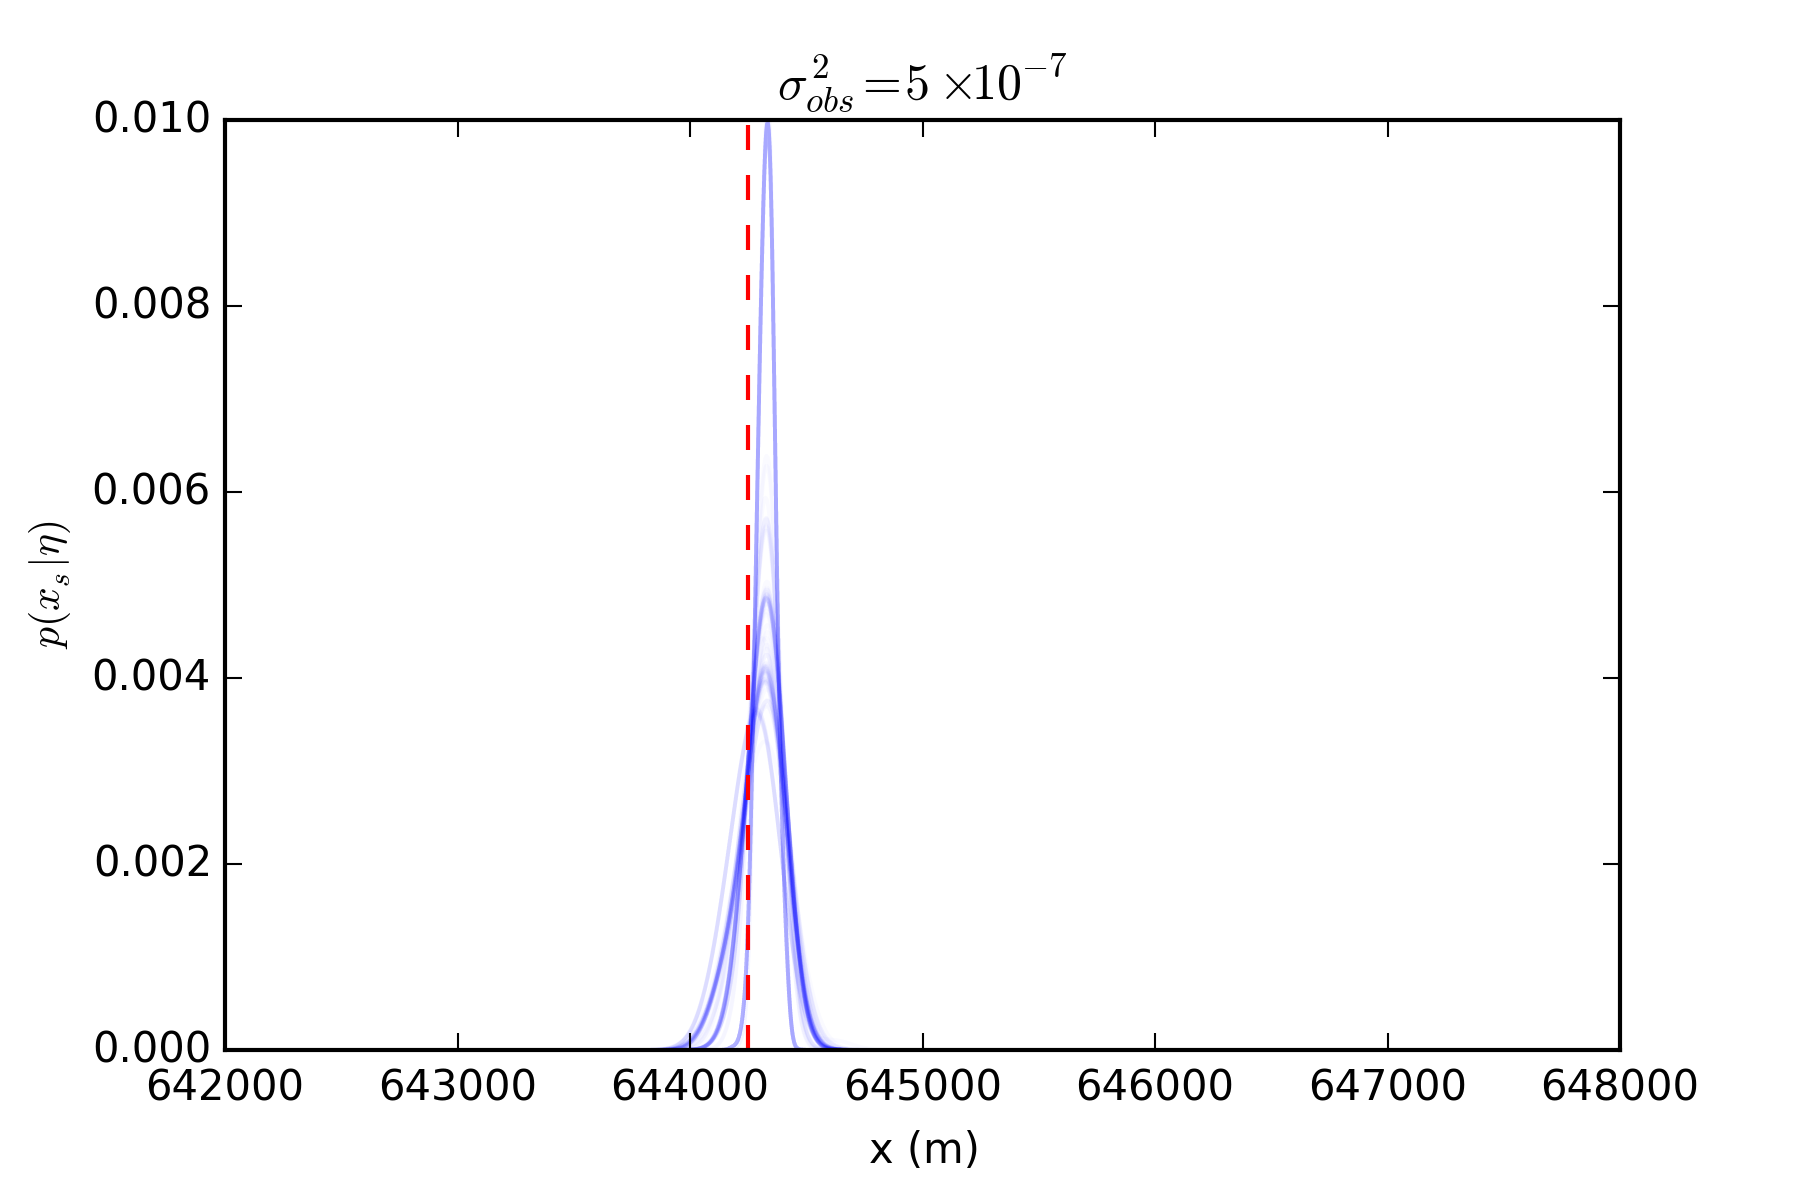
\includegraphics[width=1\textwidth]{25C_varobs_X_B.png}
  		\caption{}
  		\label{varB_x}
  	\end{subfigure}
	  	\begin{subfigure}[t]{0.5\textwidth}
	  		\centering
	  		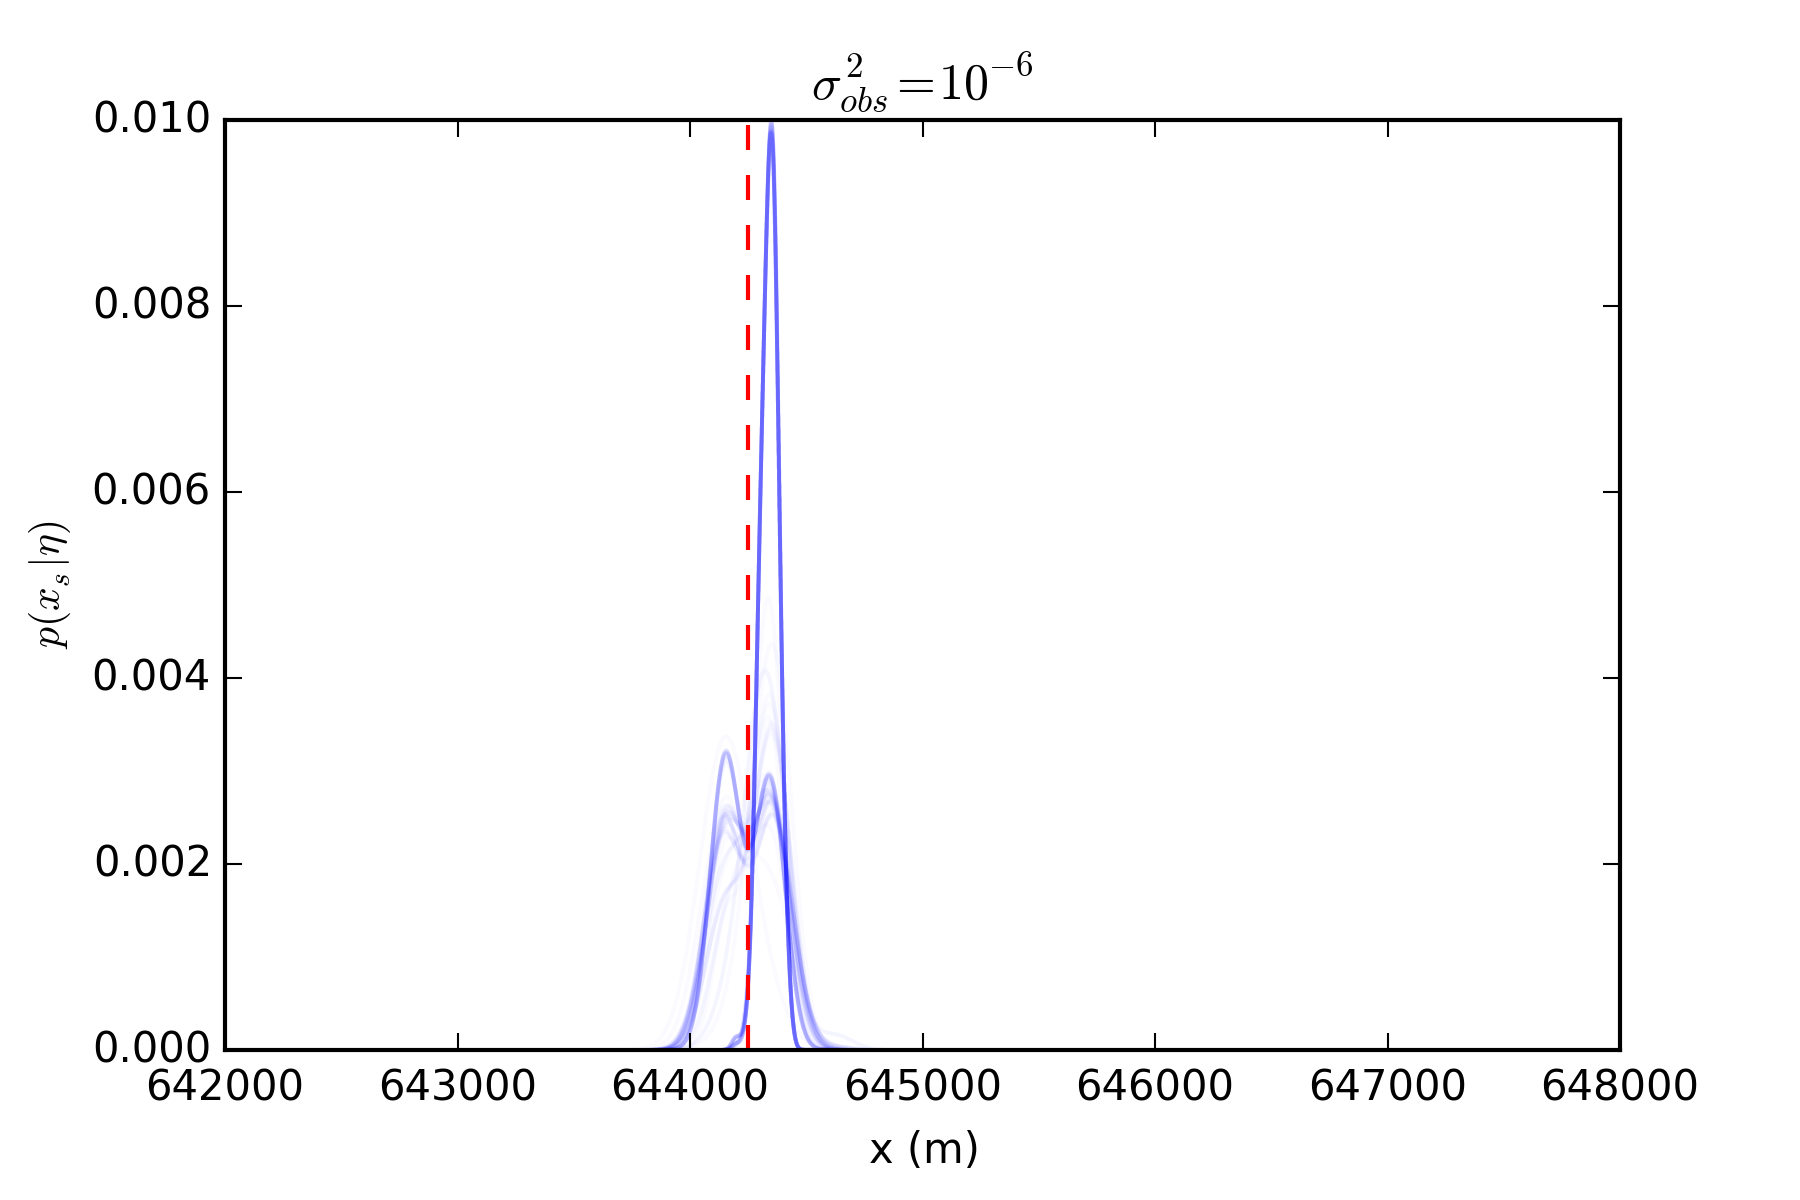
\includegraphics[width=1\textwidth]{25C_varobs_X_C.png}
	  		\caption{}
	  		\label{varC_x}
	  	\end{subfigure}%
	  	\begin{subfigure}[t]{0.5\textwidth}
	  		\centering
	  		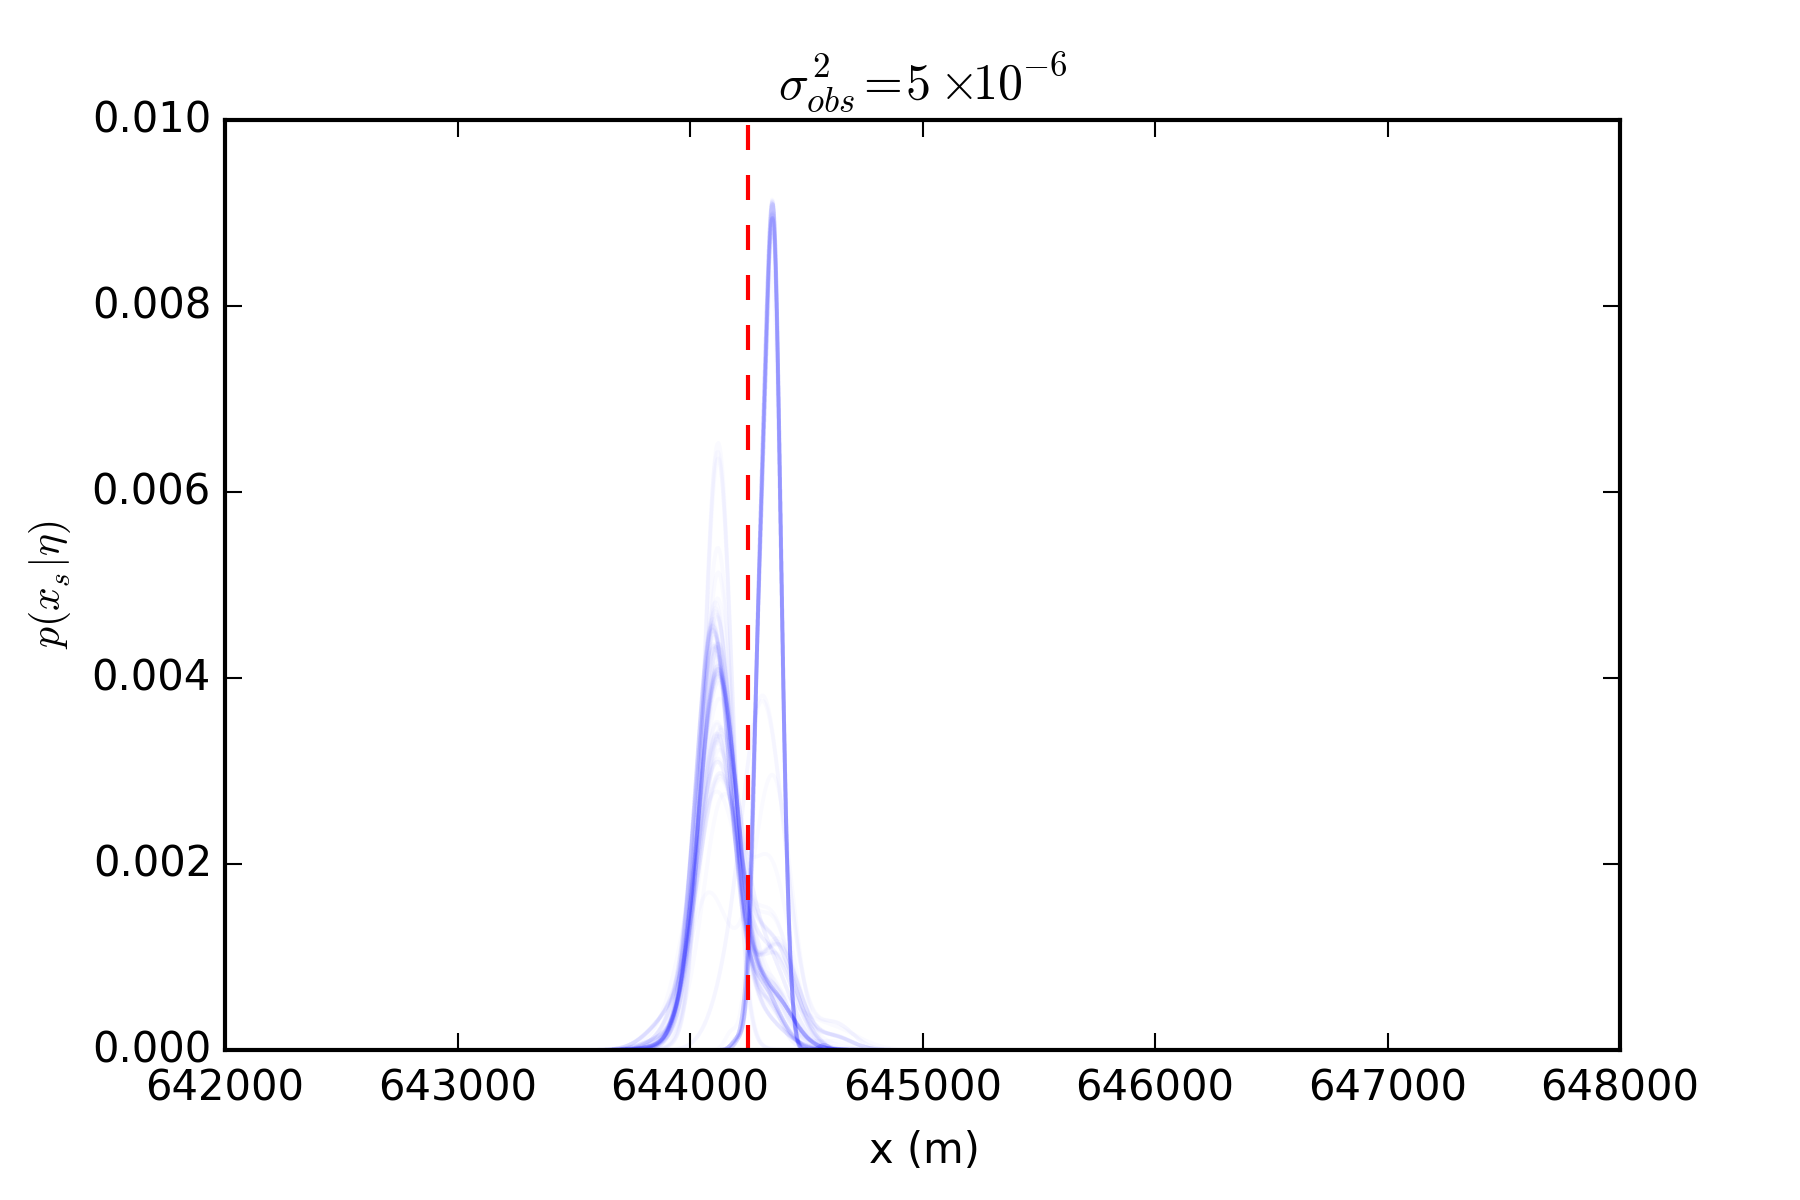
\includegraphics[width=1\textwidth]{25C_varobs_X_D.png}
	  		\caption{}
	  		\label{varD_x}
	  	\end{subfigure}
	   	\begin{subfigure}[t]{0.5\textwidth}
	   		\centering
	   		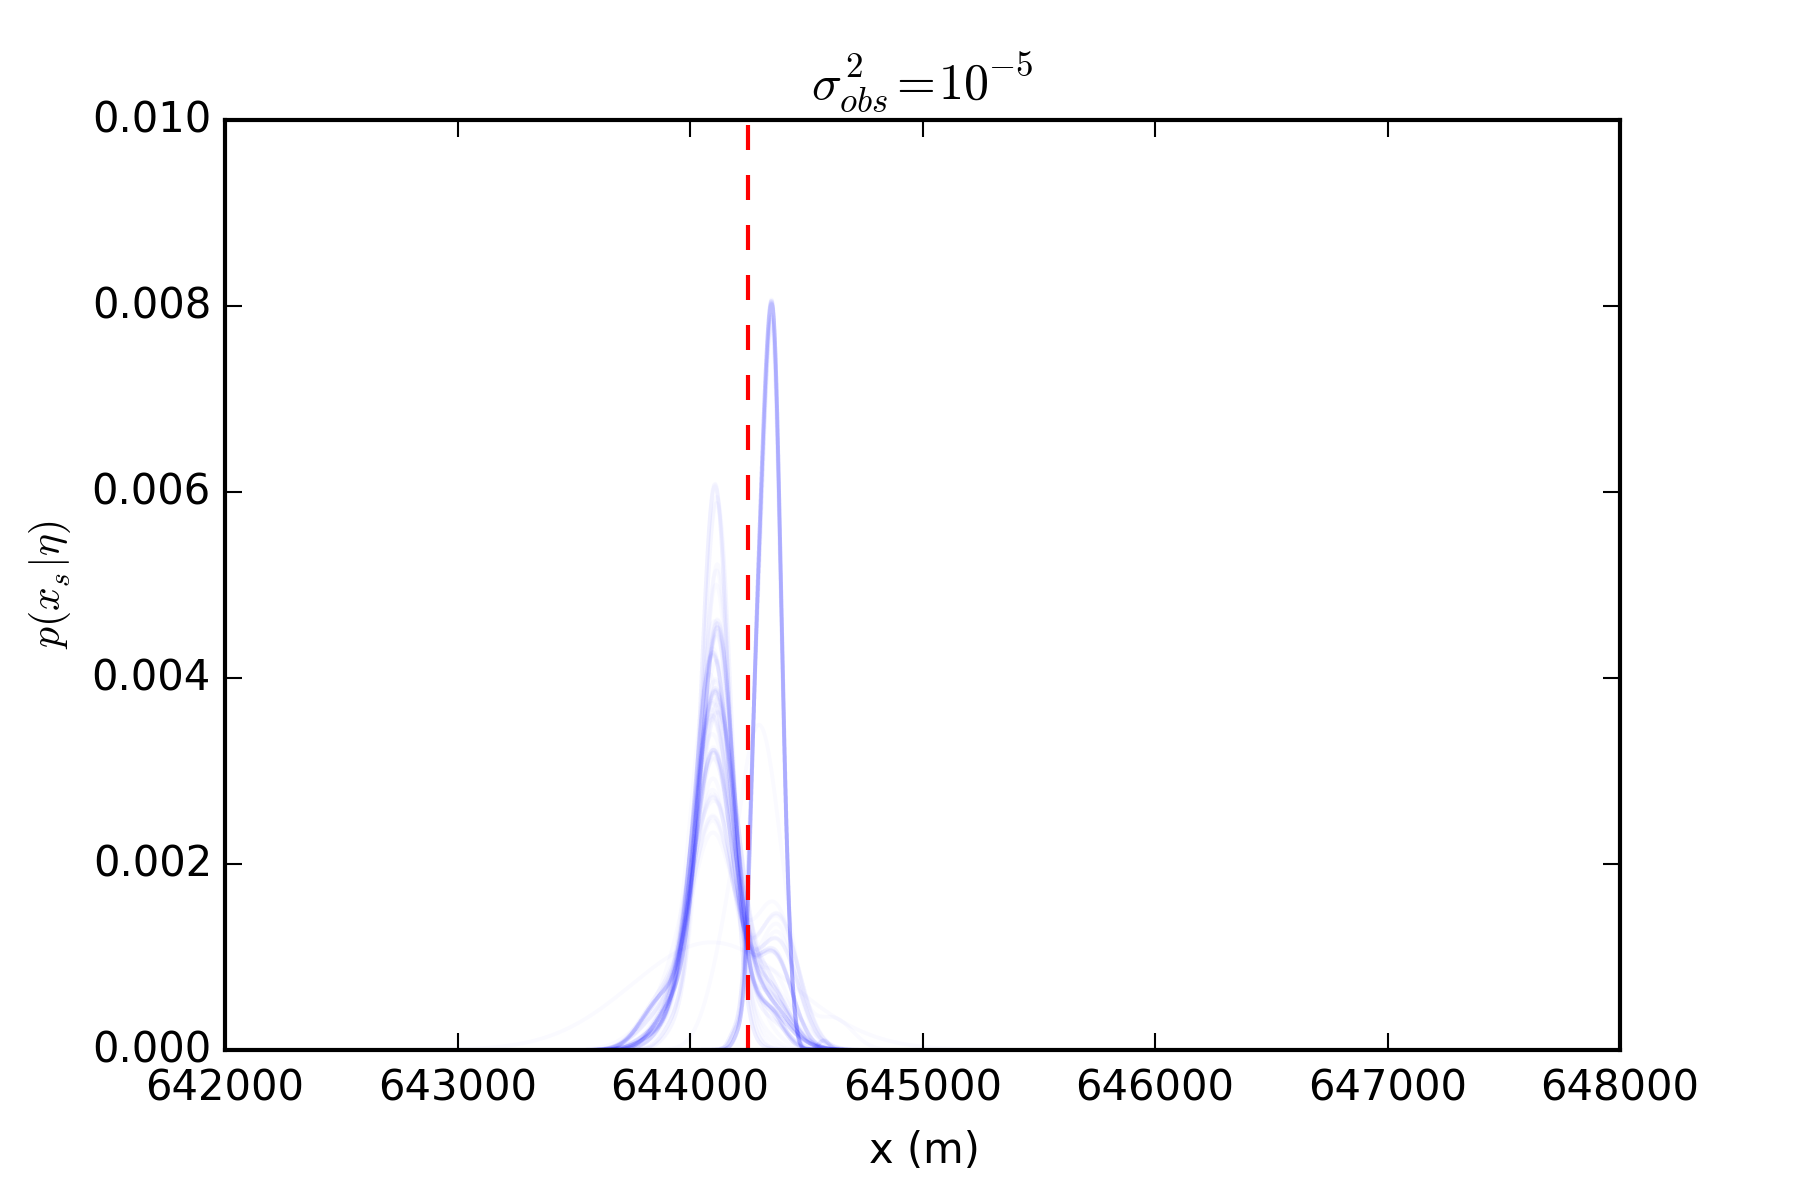
\includegraphics[width=1\textwidth]{25C_varobs_X_E.png}
	   		\caption{}
	   		\label{varE_x}
	   	\end{subfigure}%
	   	\begin{subfigure}[t]{0.5\textwidth}
	   		\centering
	   		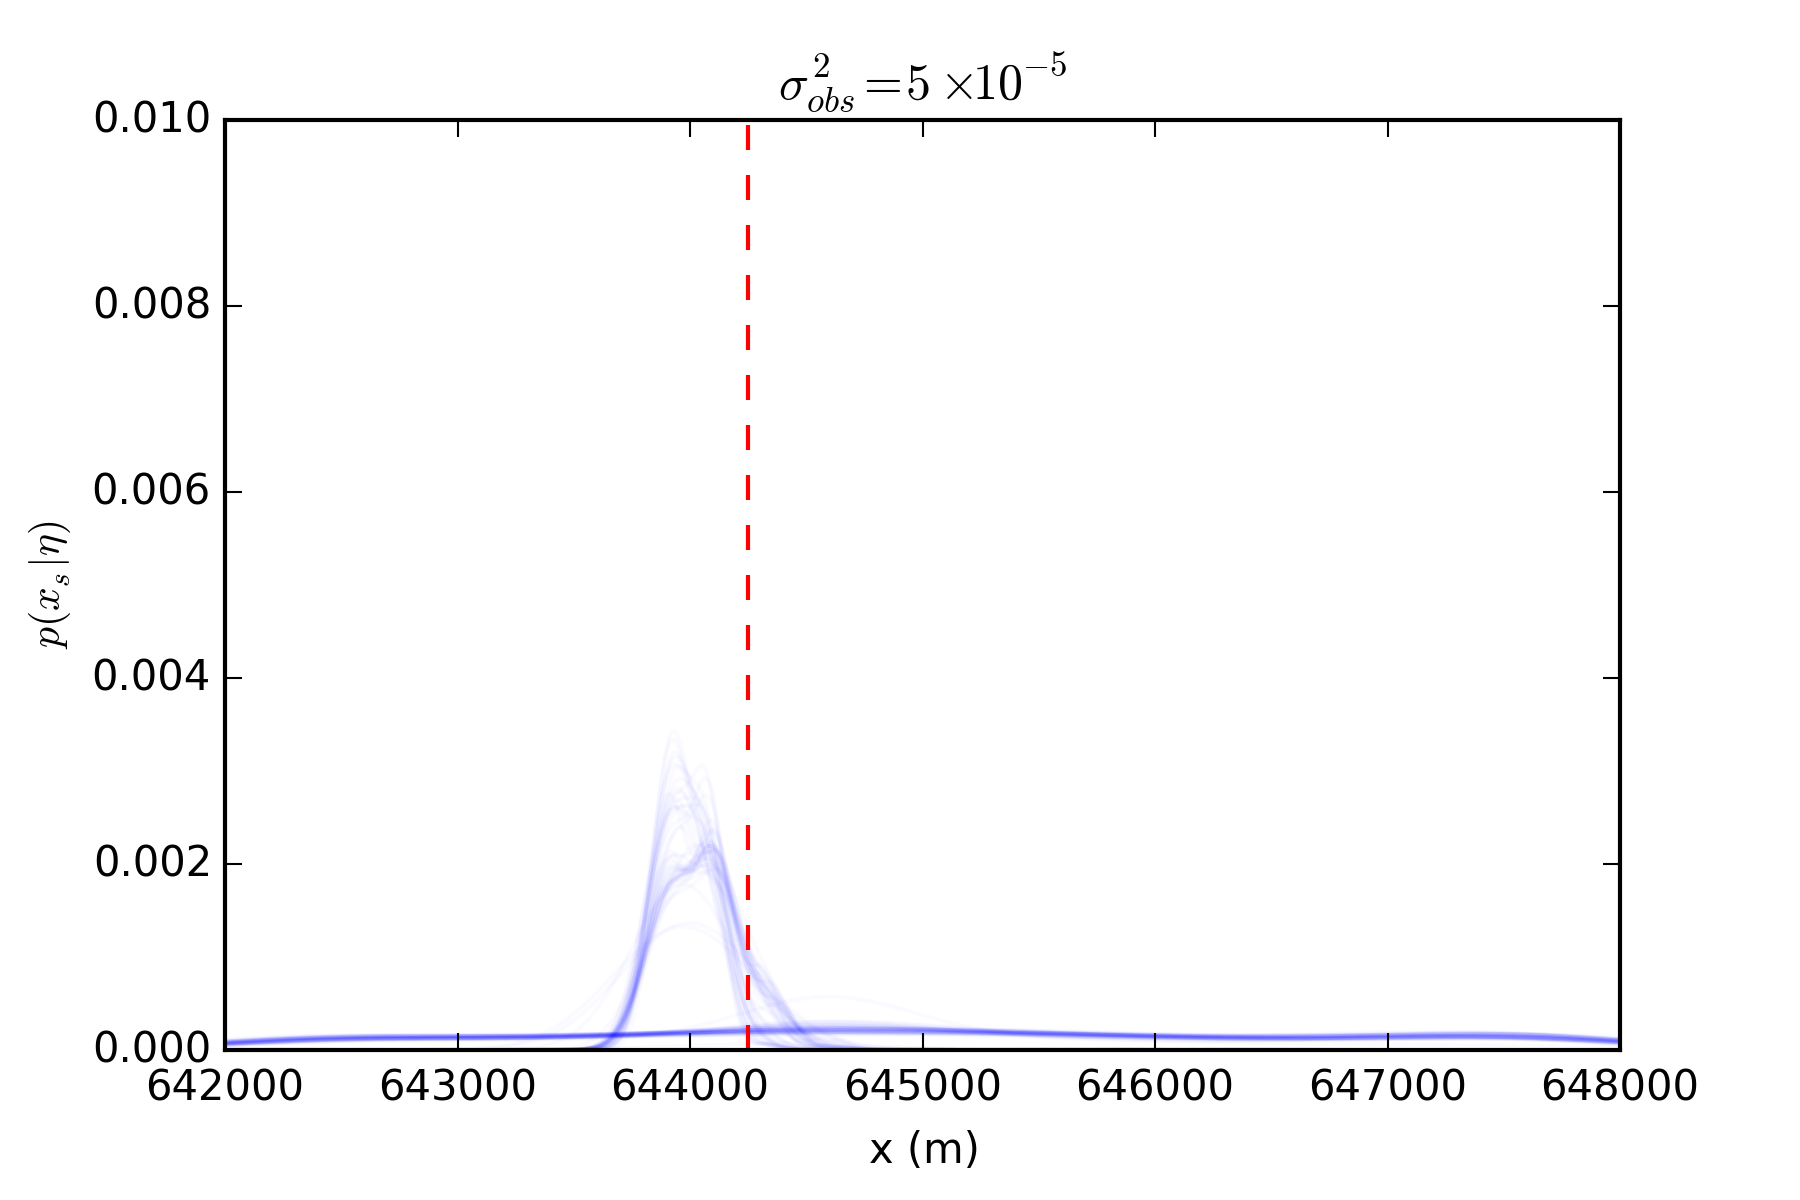
\includegraphics[width=1\textwidth]{25C_varobs_X_F.png}
	   		\caption{}
	   		\label{varF_x}
	   	\end{subfigure}
	   	\caption{Analyse paramétrique sur la variance d'observation $\varObs$ pour le cas-test Beaune (25 capteurs): localisation en $x$ de la source}
	   	\label{fig_25C_analyse_varobs_x}

  \end{figure}
  
  
  
  \begin{figure}[p!]
  	\centering
  	\begin{subfigure}[t]{0.5\textwidth}
  		\centering
  		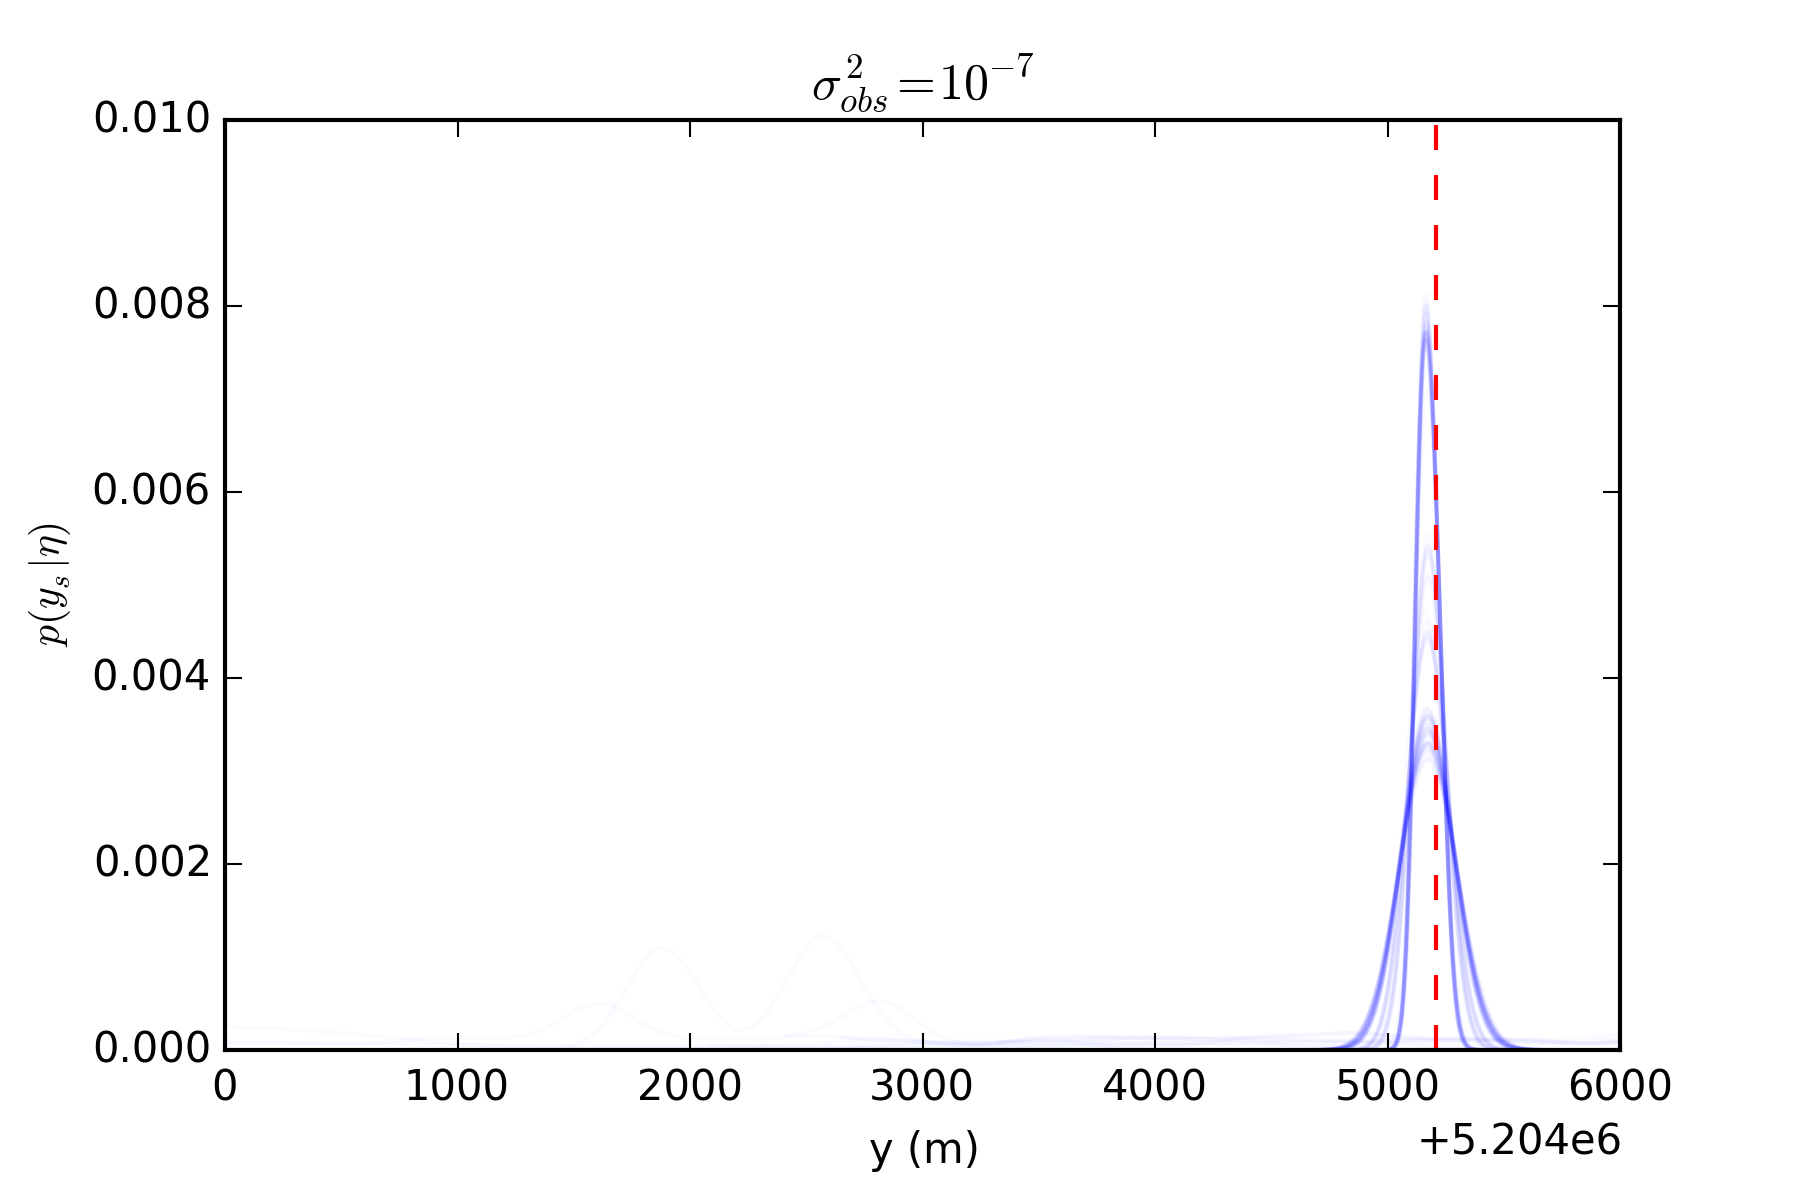
\includegraphics[width=1\textwidth]{25C_varobs_Y_A.png}
  		\caption{}
  		\label{varA_y}
  	\end{subfigure}%
  	\begin{subfigure}[t]{0.5\textwidth}
  		\centering
  		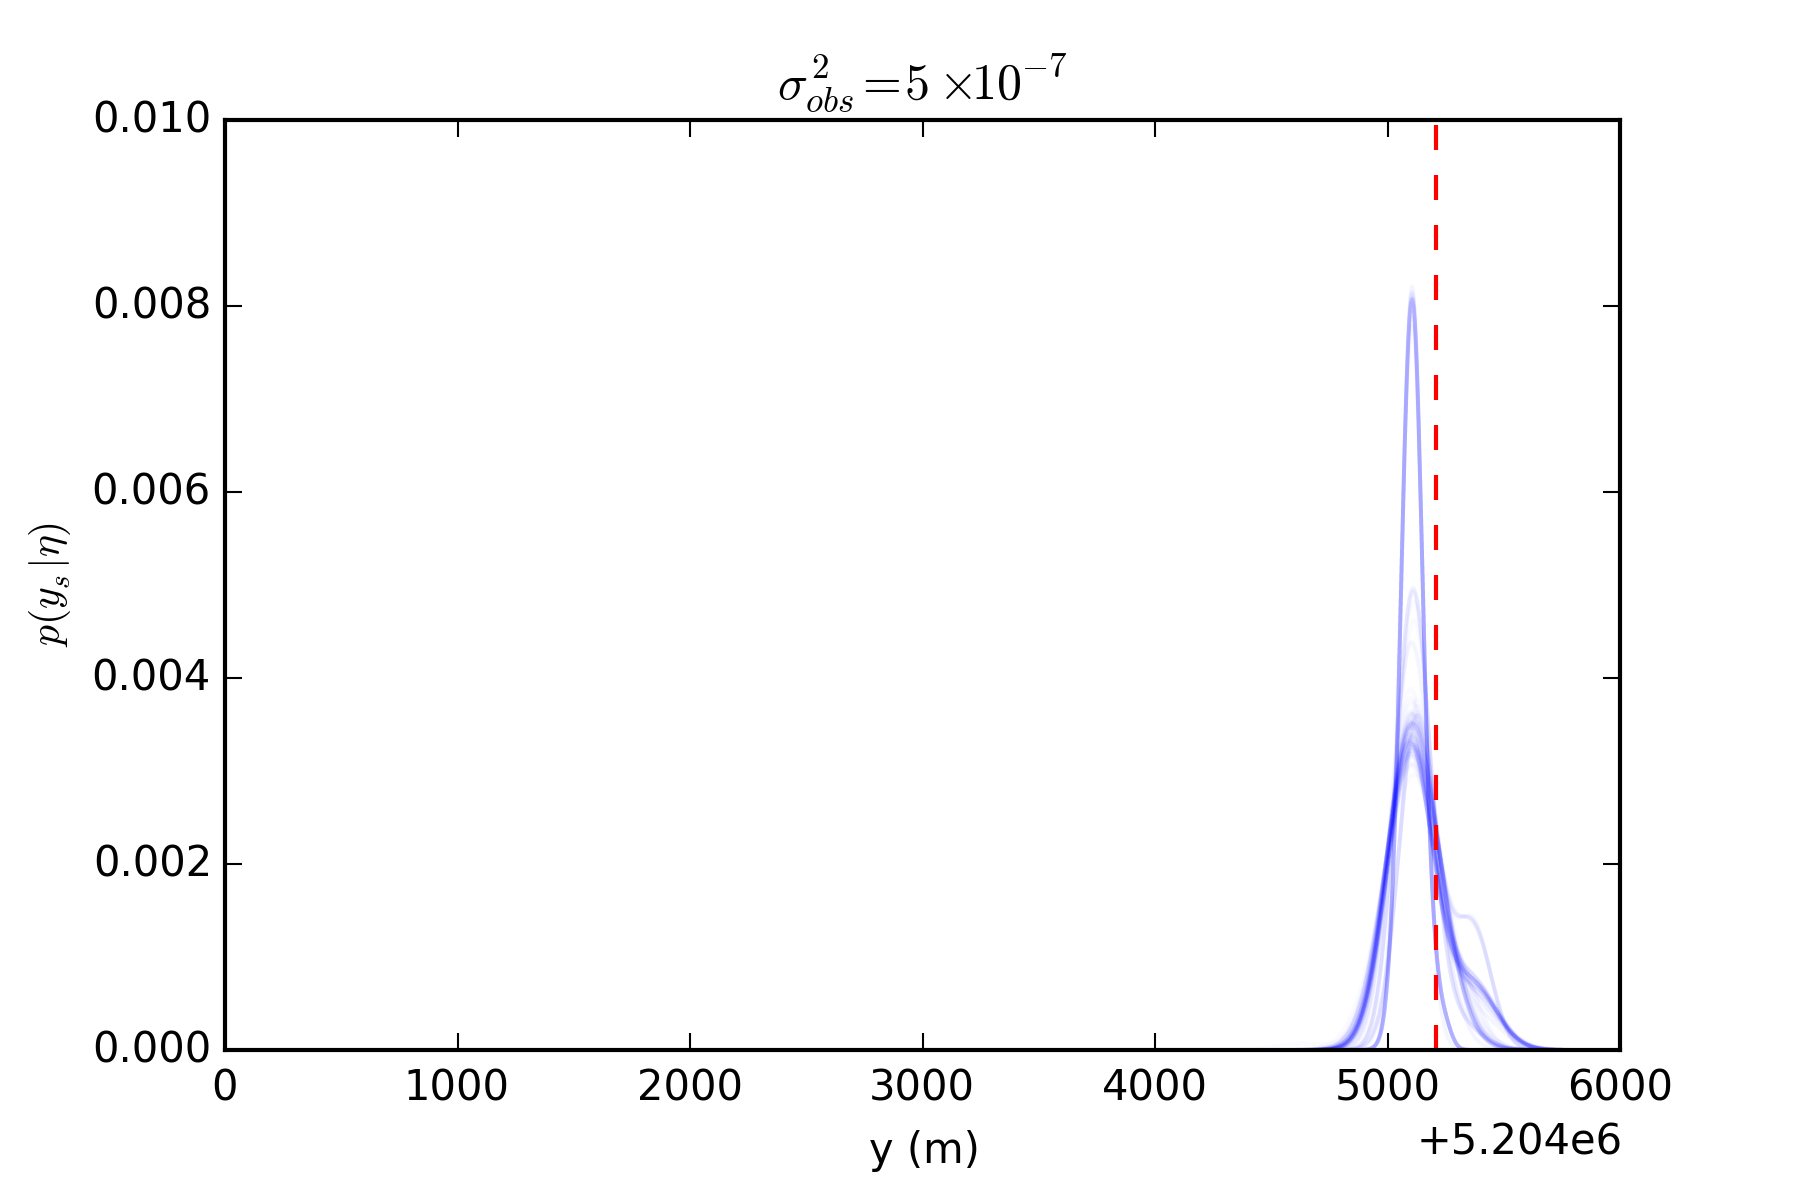
\includegraphics[width=1\textwidth]{25C_varobs_Y_B.png}
  		\caption{}
  		\label{varB_y}
  	\end{subfigure}
  	\begin{subfigure}[t]{0.5\textwidth}
  		\centering
  		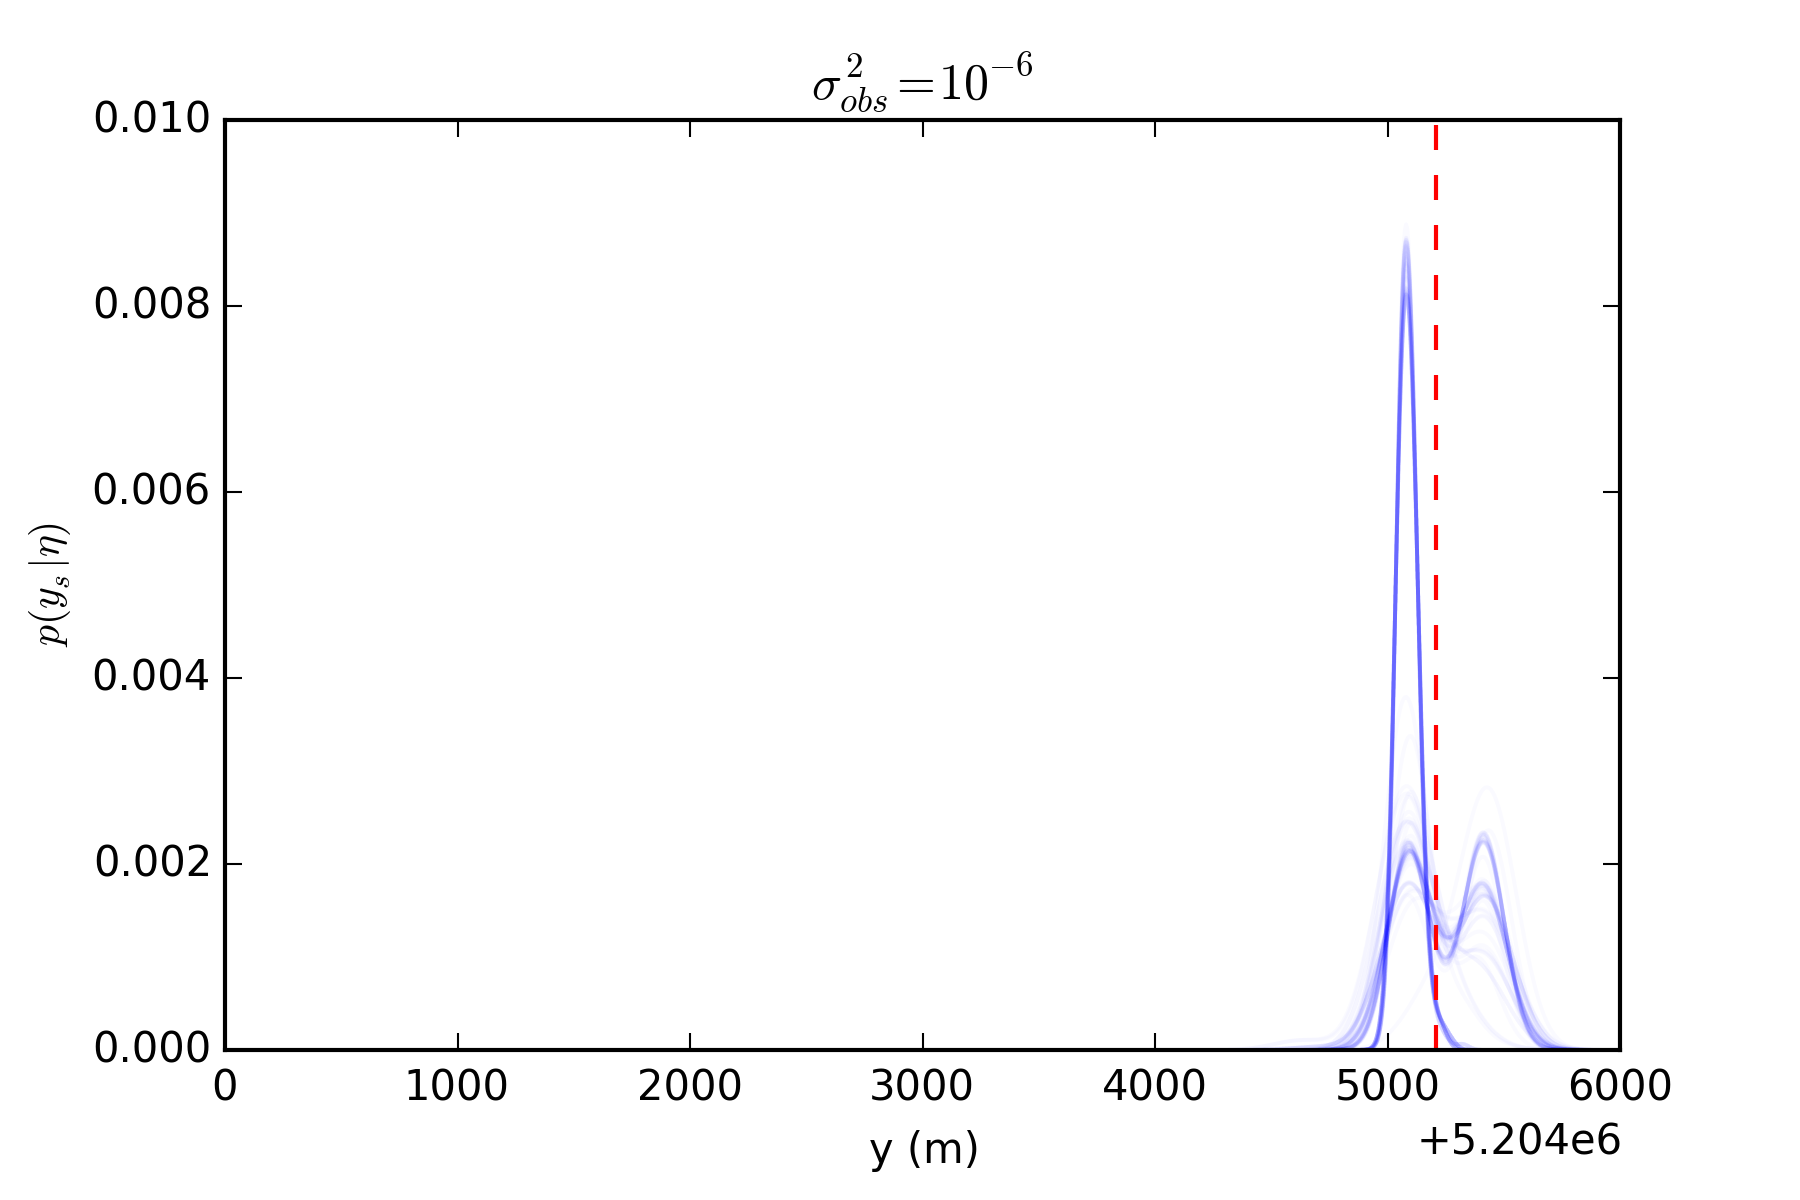
\includegraphics[width=1\textwidth]{25C_varobs_Y_C.png}
  		\caption{}
  		\label{varC_y}
  	\end{subfigure}%
  	\begin{subfigure}[t]{0.5\textwidth}
  		\centering
  		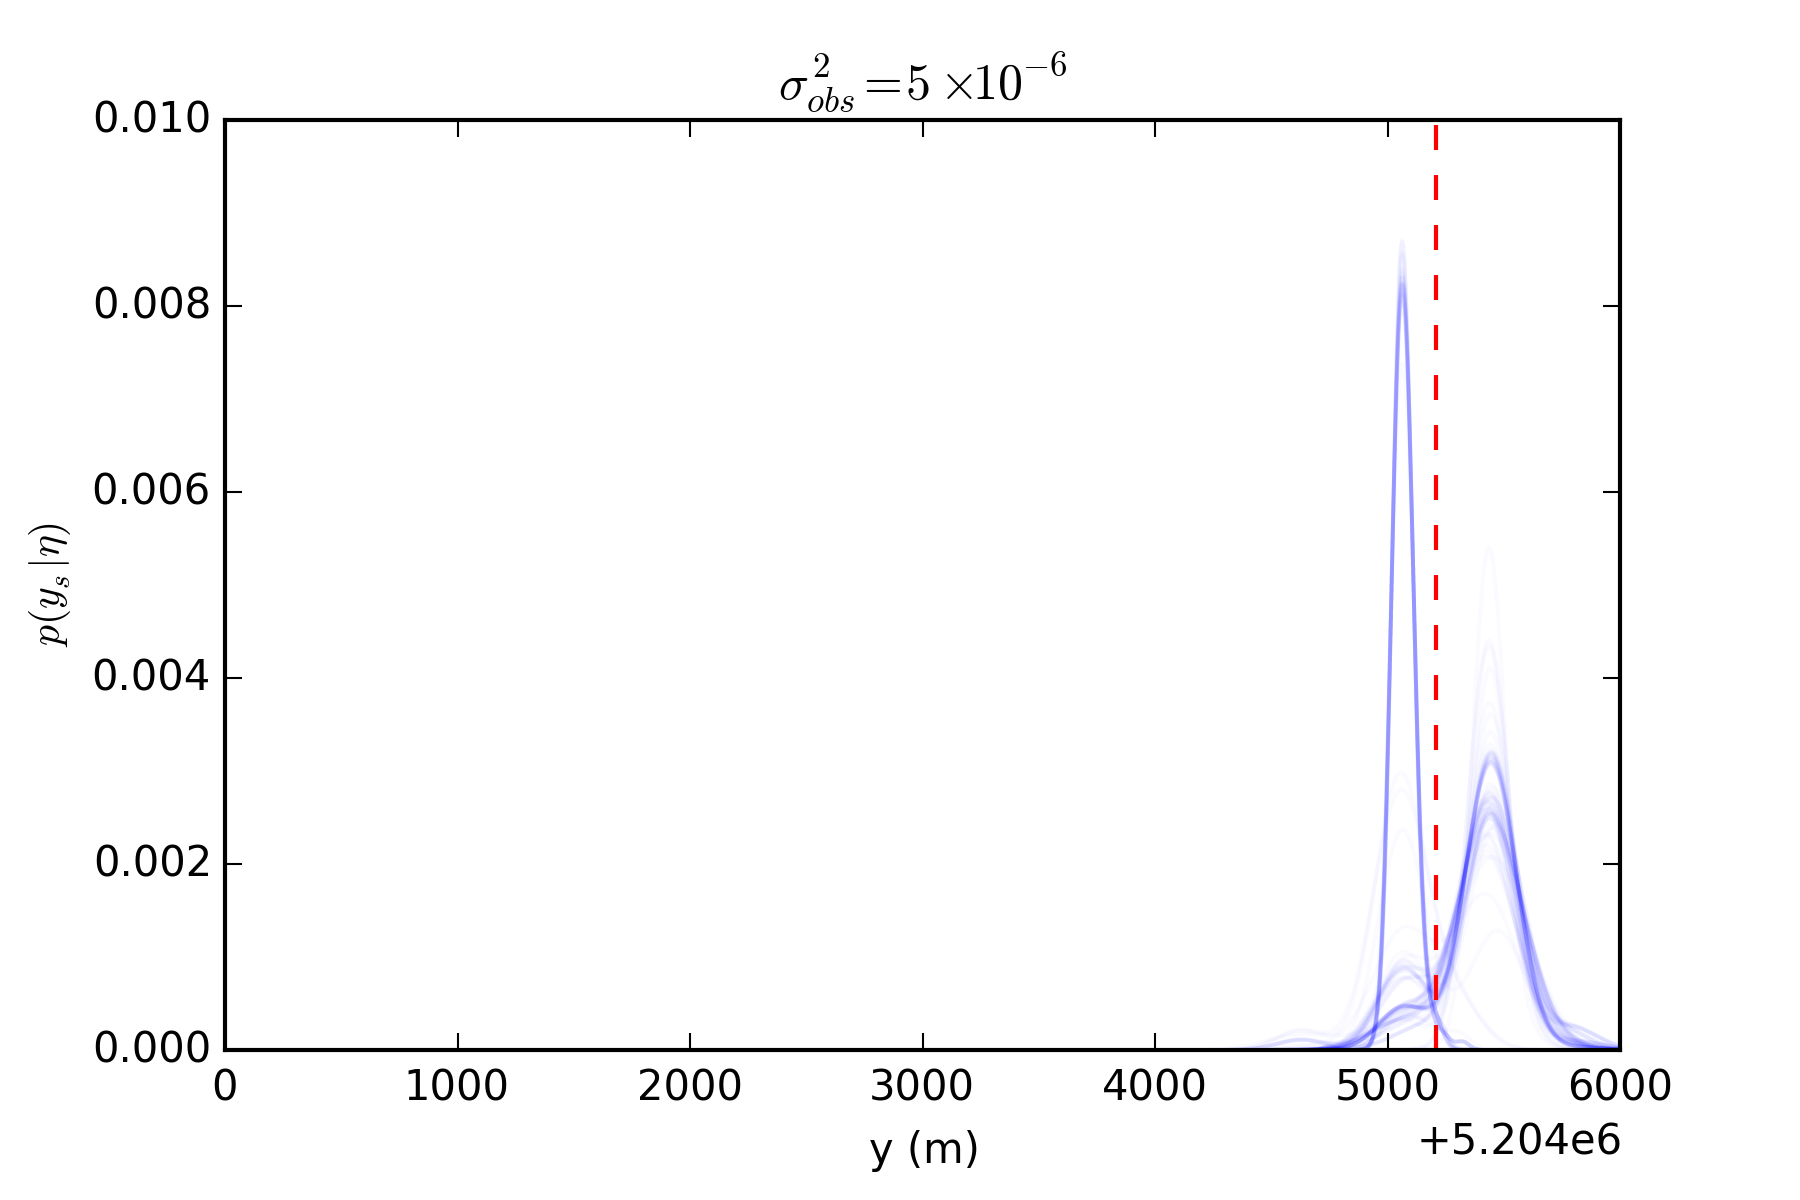
\includegraphics[width=1\textwidth]{25C_varobs_Y_D.png}
  		\caption{}
  		\label{varD_y}
  	\end{subfigure}
  	\begin{subfigure}[t]{0.5\textwidth}
  		\centering
  		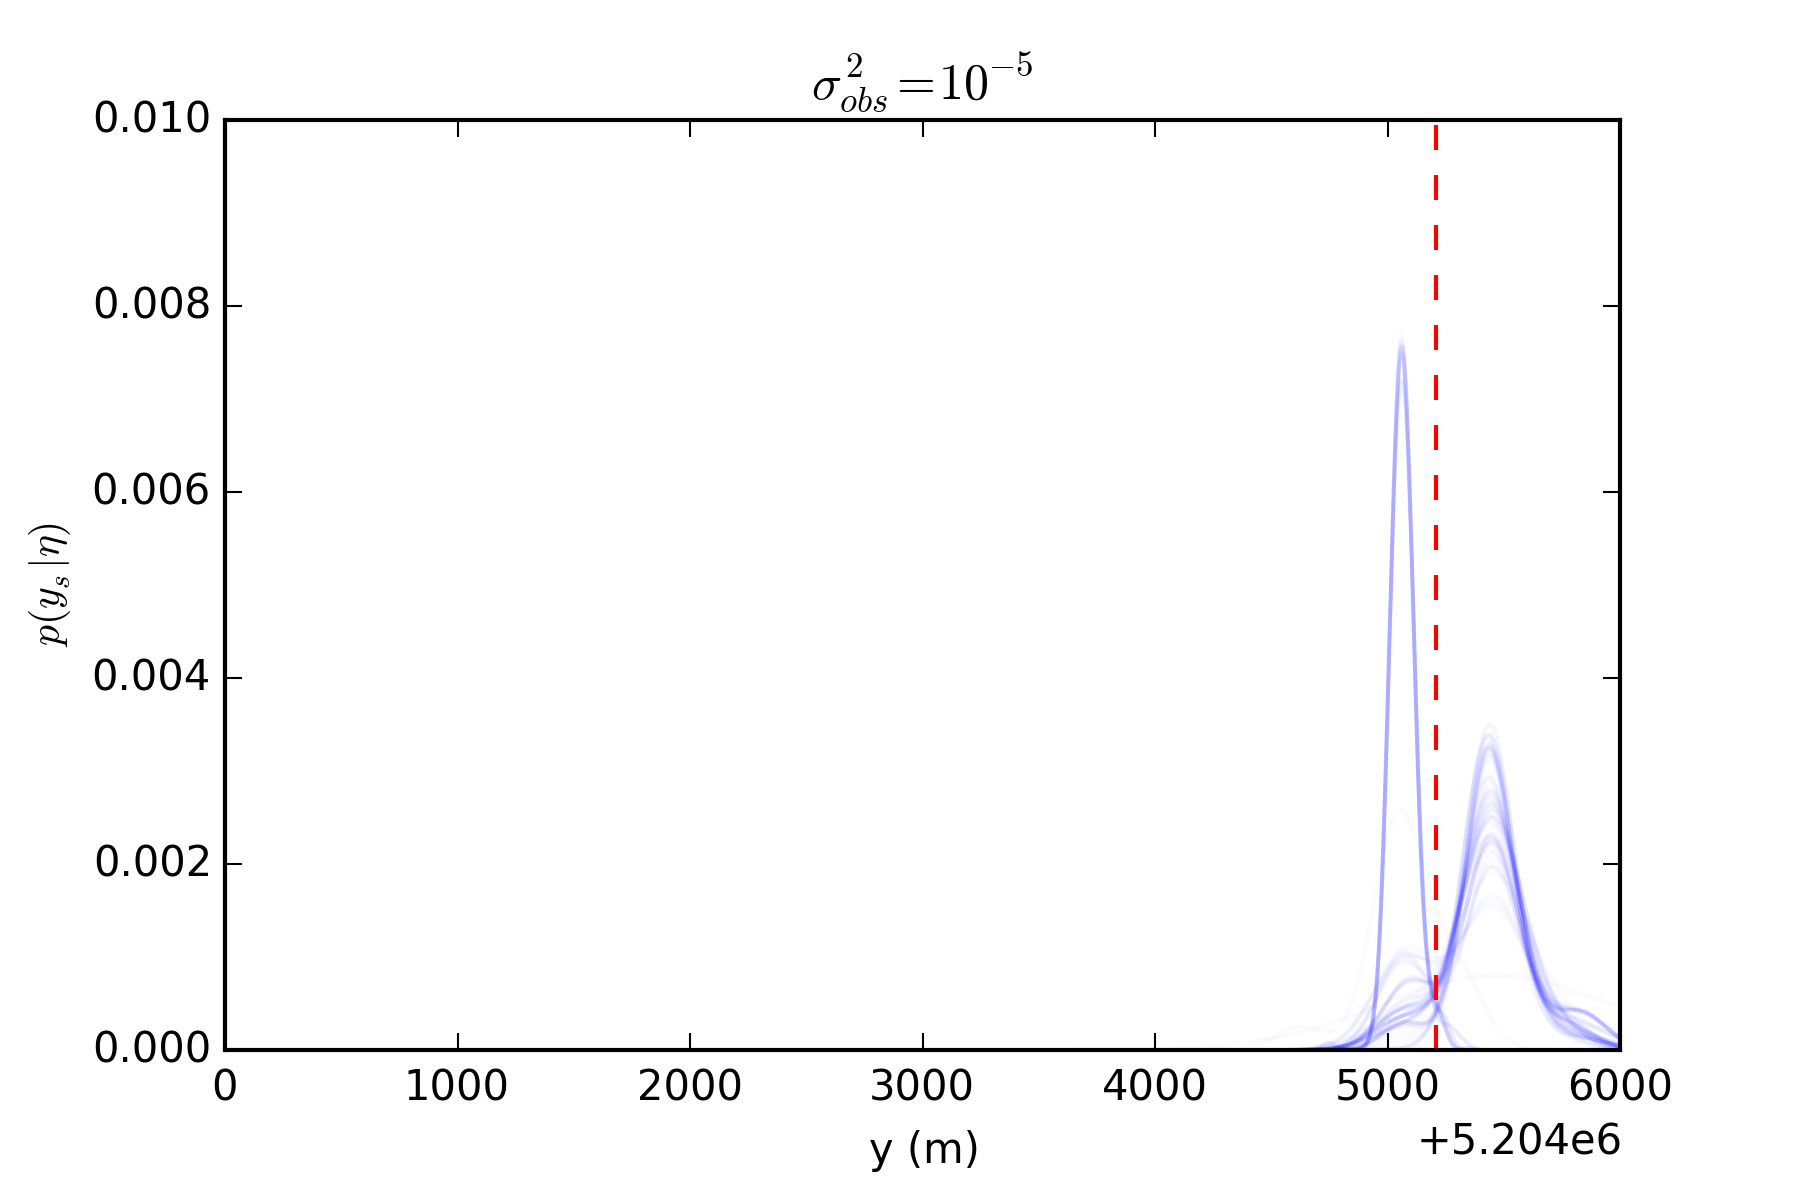
\includegraphics[width=1\textwidth]{25C_varobs_Y_E.png}
  		\caption{}
  		\label{varE_y}
  	\end{subfigure}%
  	\begin{subfigure}[t]{0.5\textwidth}
  		\centering
  		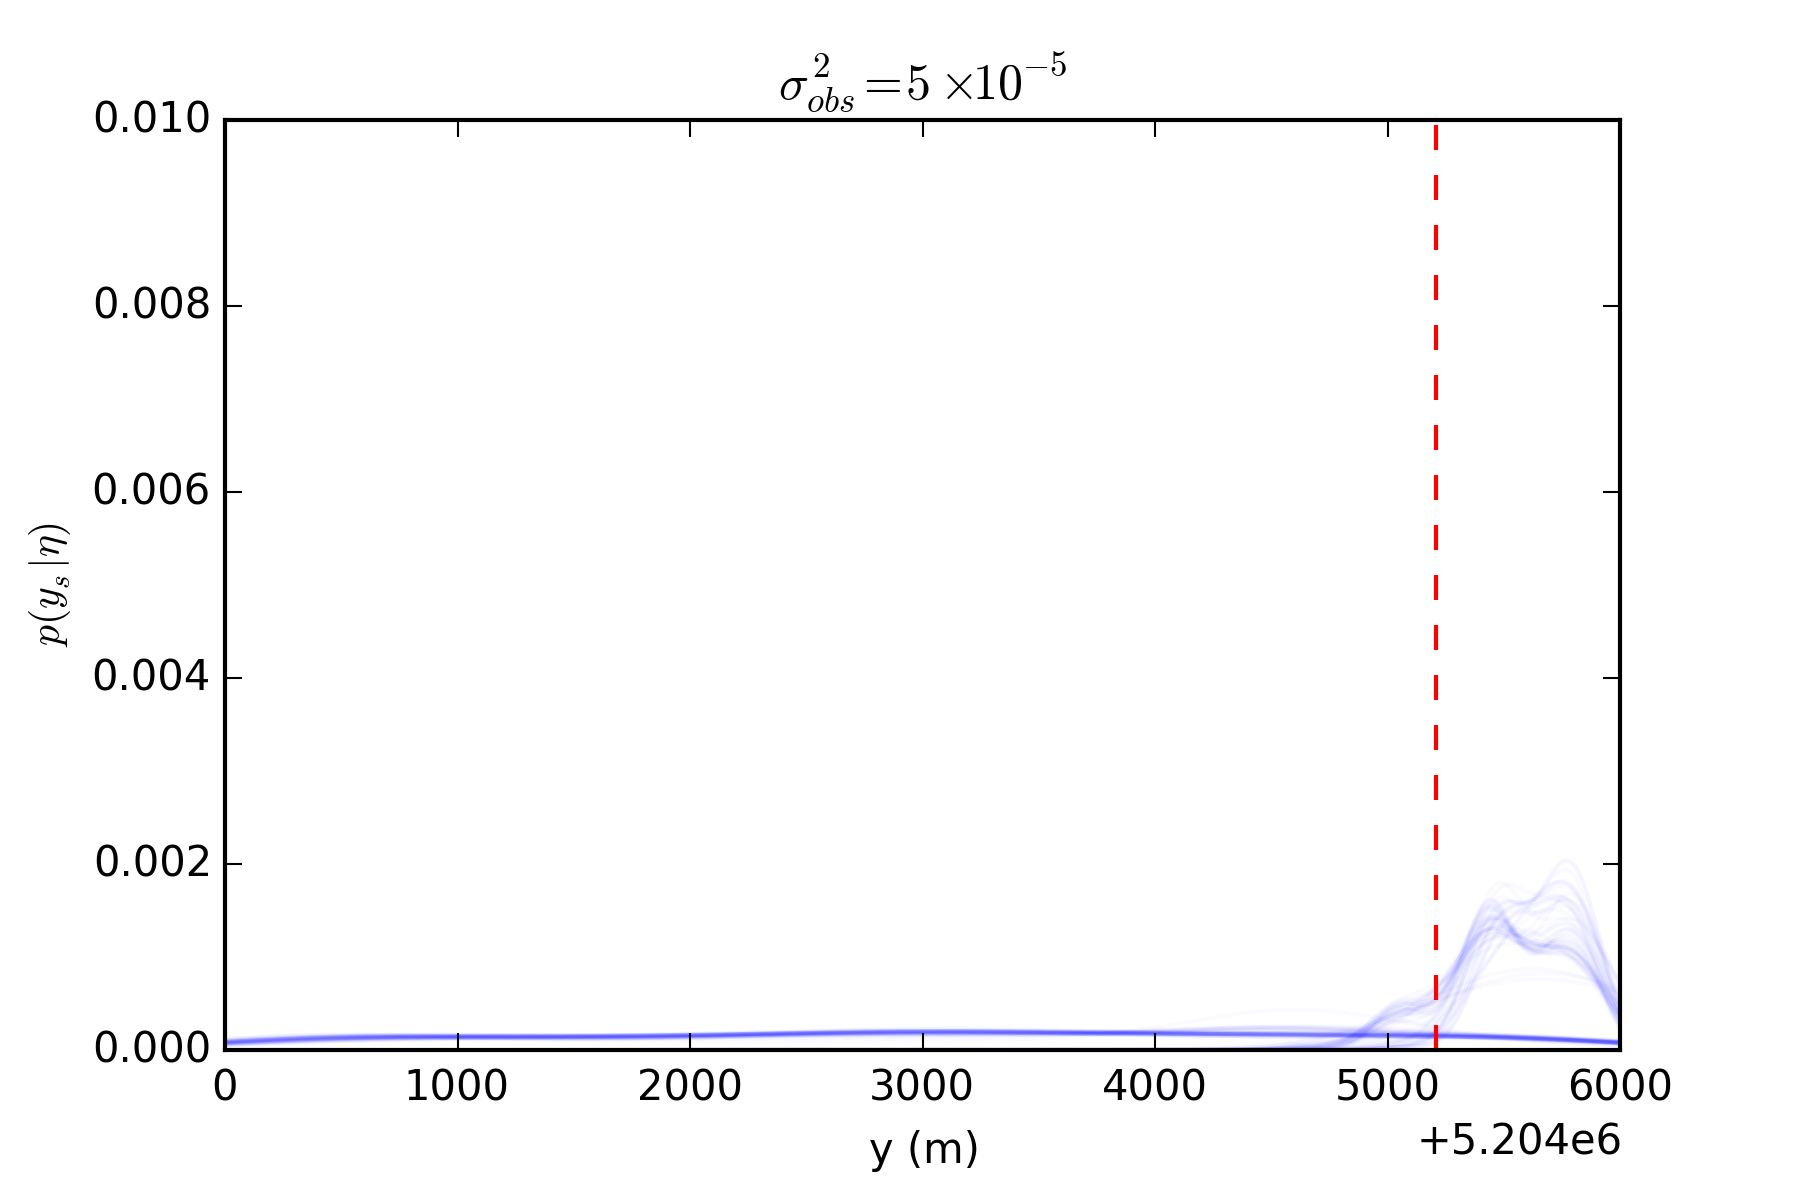
\includegraphics[width=1\textwidth]{25C_varobs_Y_F.png}
  		\caption{}
  		\label{varF_y}
  	\end{subfigure}
  	\caption{Analyse paramétrique sur la variance d'observation $\varObs$ pour le cas-test Beaune (25 capteurs): localisation en $y$ de la source}
  	\label{fig_25C_analyse_varobs_y}
  	
  \end{figure}
  
  
  \begin{figure}[p!]
  	\centering
  	\begin{subfigure}[t]{0.5\textwidth}
  		\centering
  		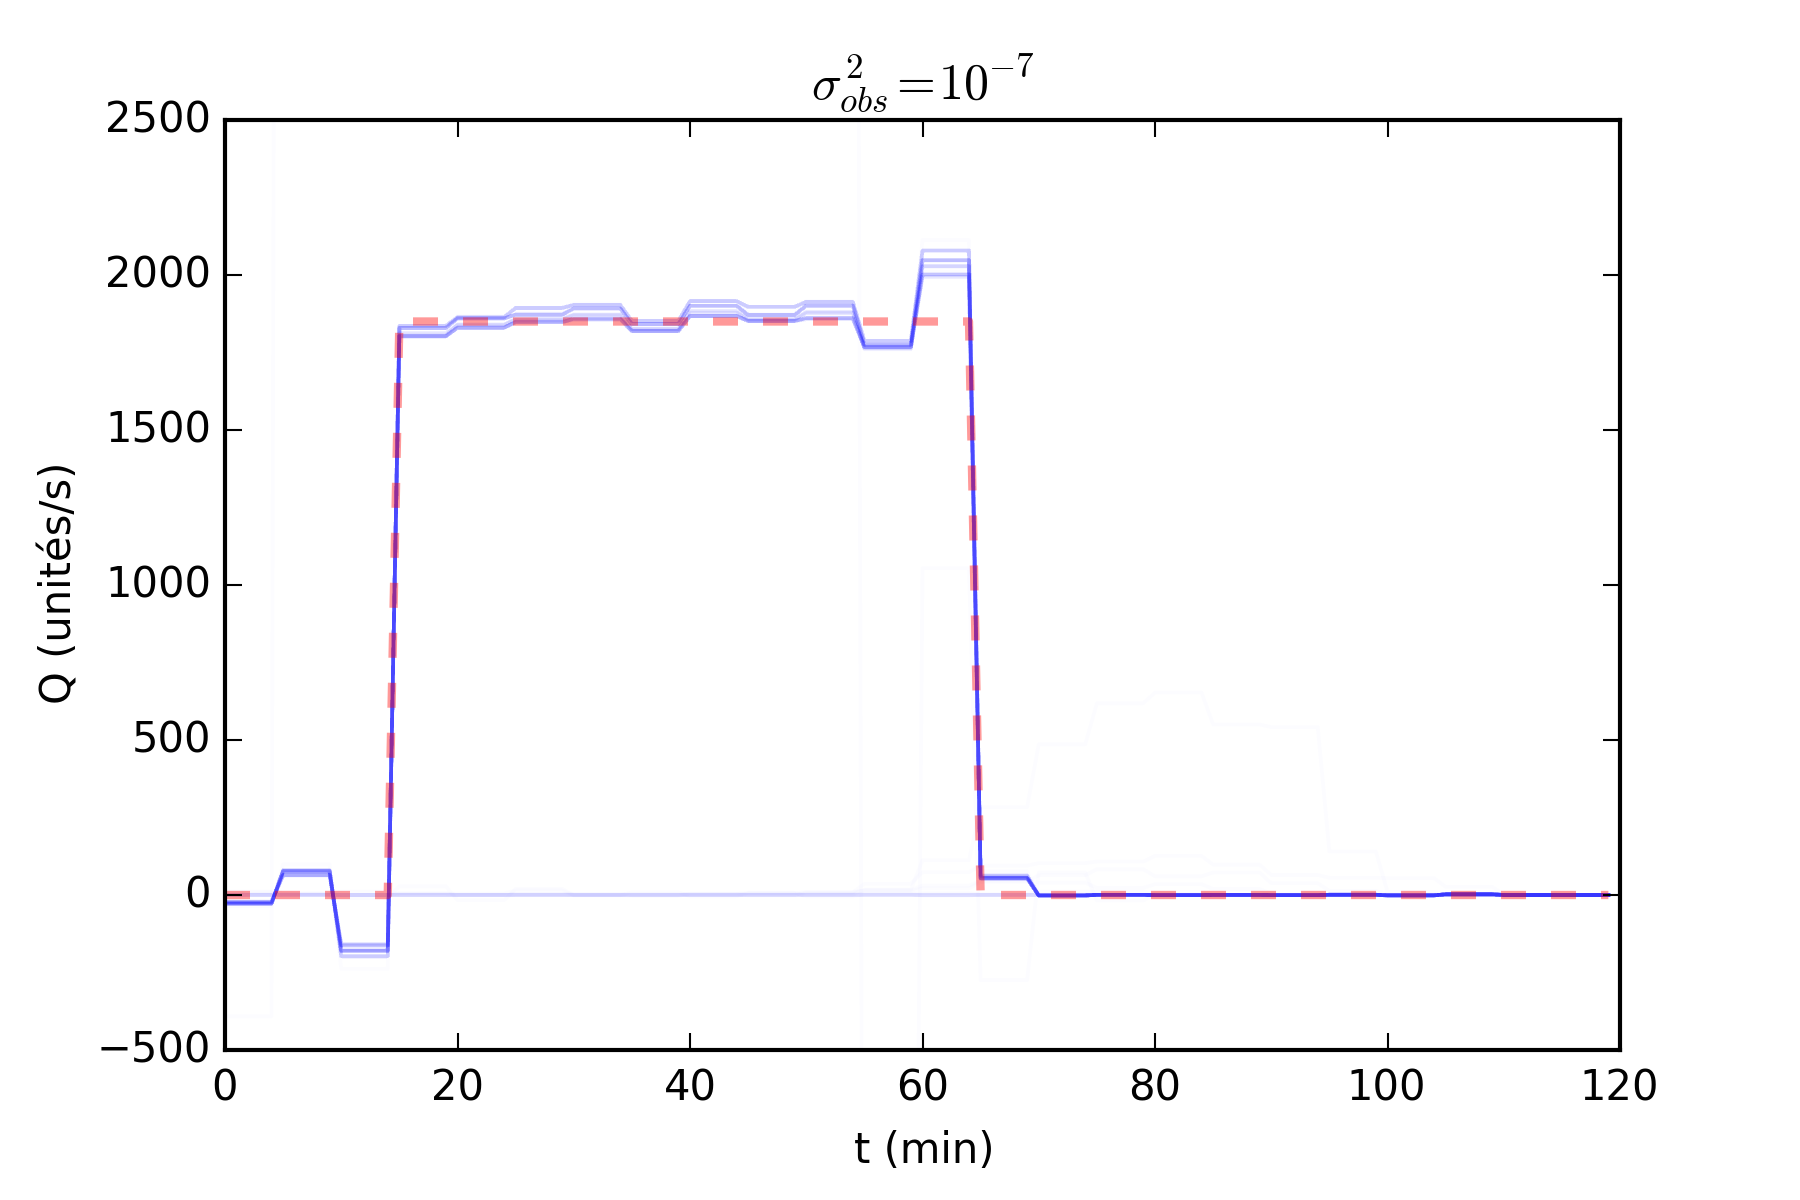
\includegraphics[width=1\textwidth]{25C_varobs_Q_A.png}
  		\caption{}
  		\label{varA_q}
  	\end{subfigure}%
  	\begin{subfigure}[t]{0.5\textwidth}
  		\centering
  		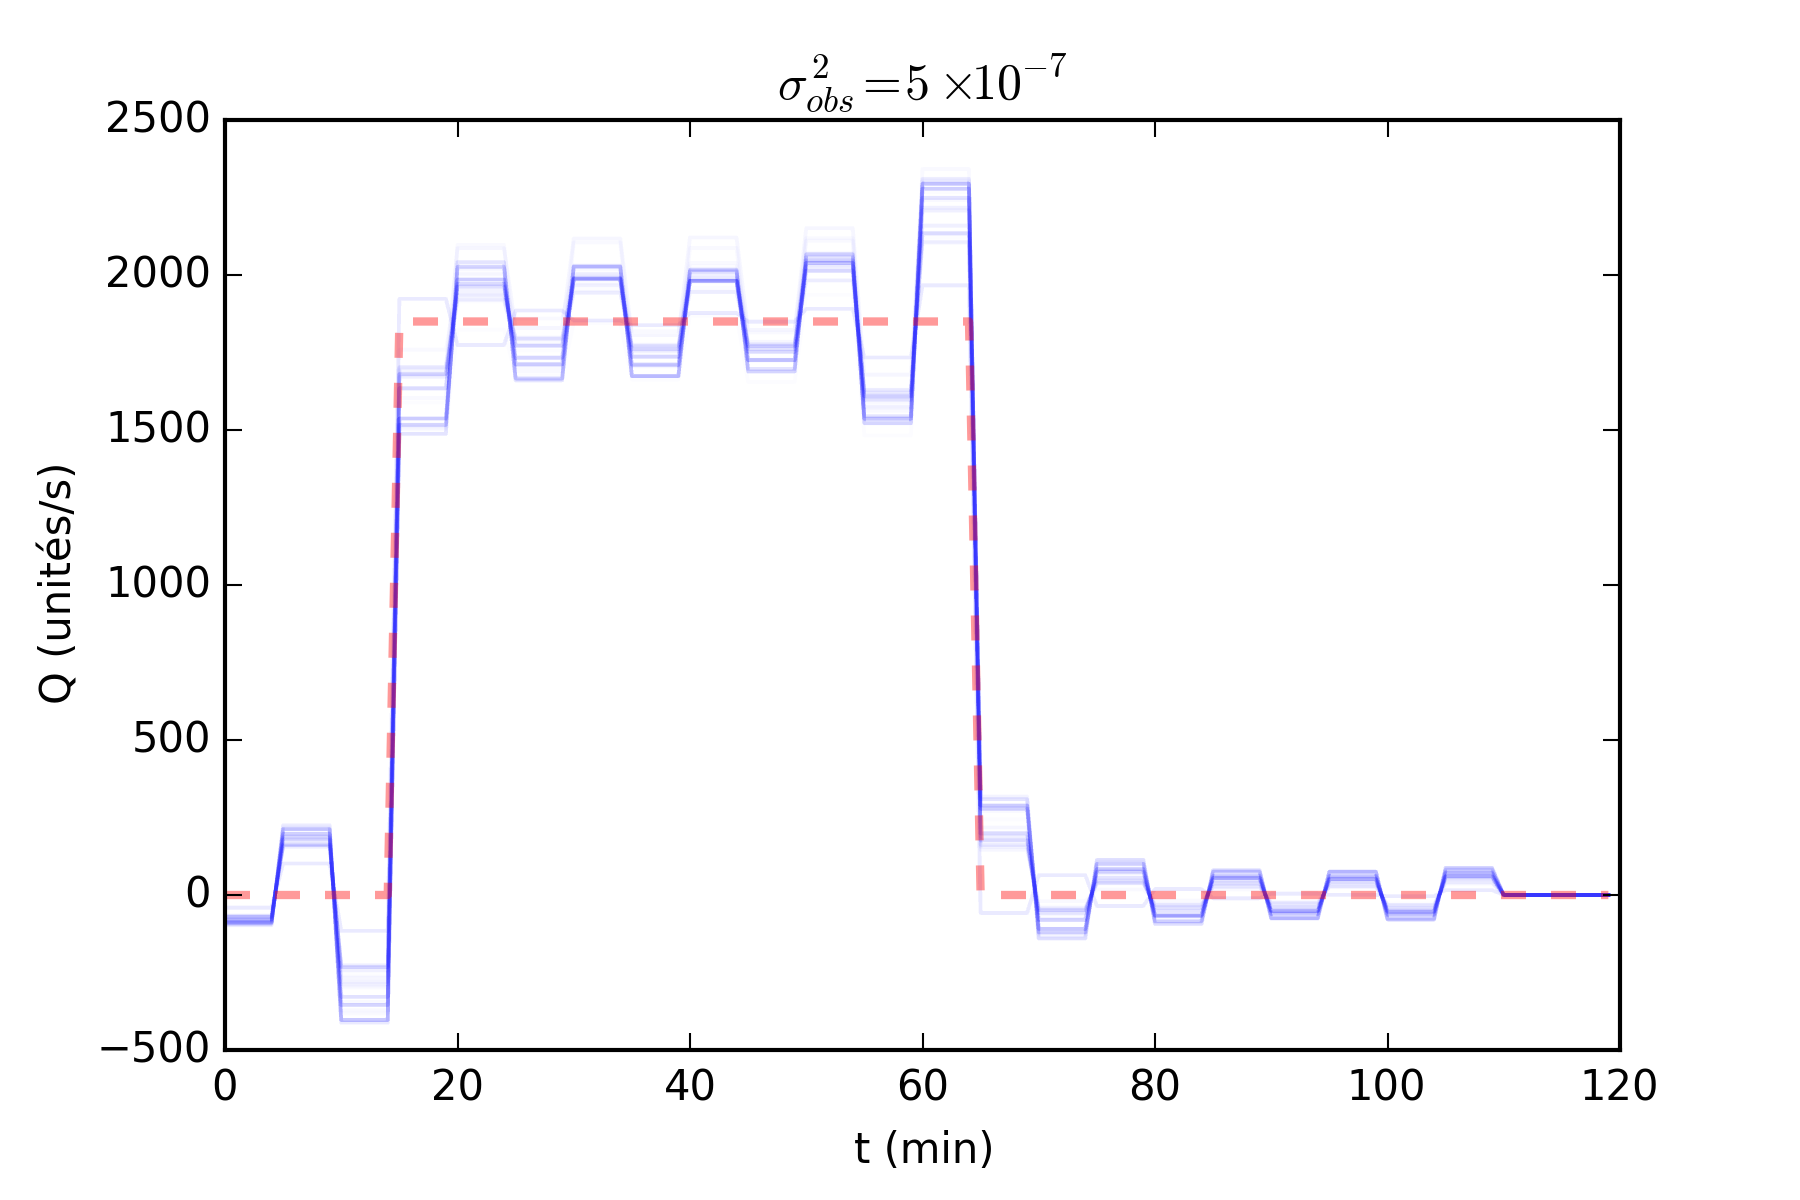
\includegraphics[width=1\textwidth]{25C_varobs_Q_B.png}
  		\caption{}
  		\label{varB_q}
  	\end{subfigure}
  	\begin{subfigure}[t]{0.5\textwidth}
  		\centering
  		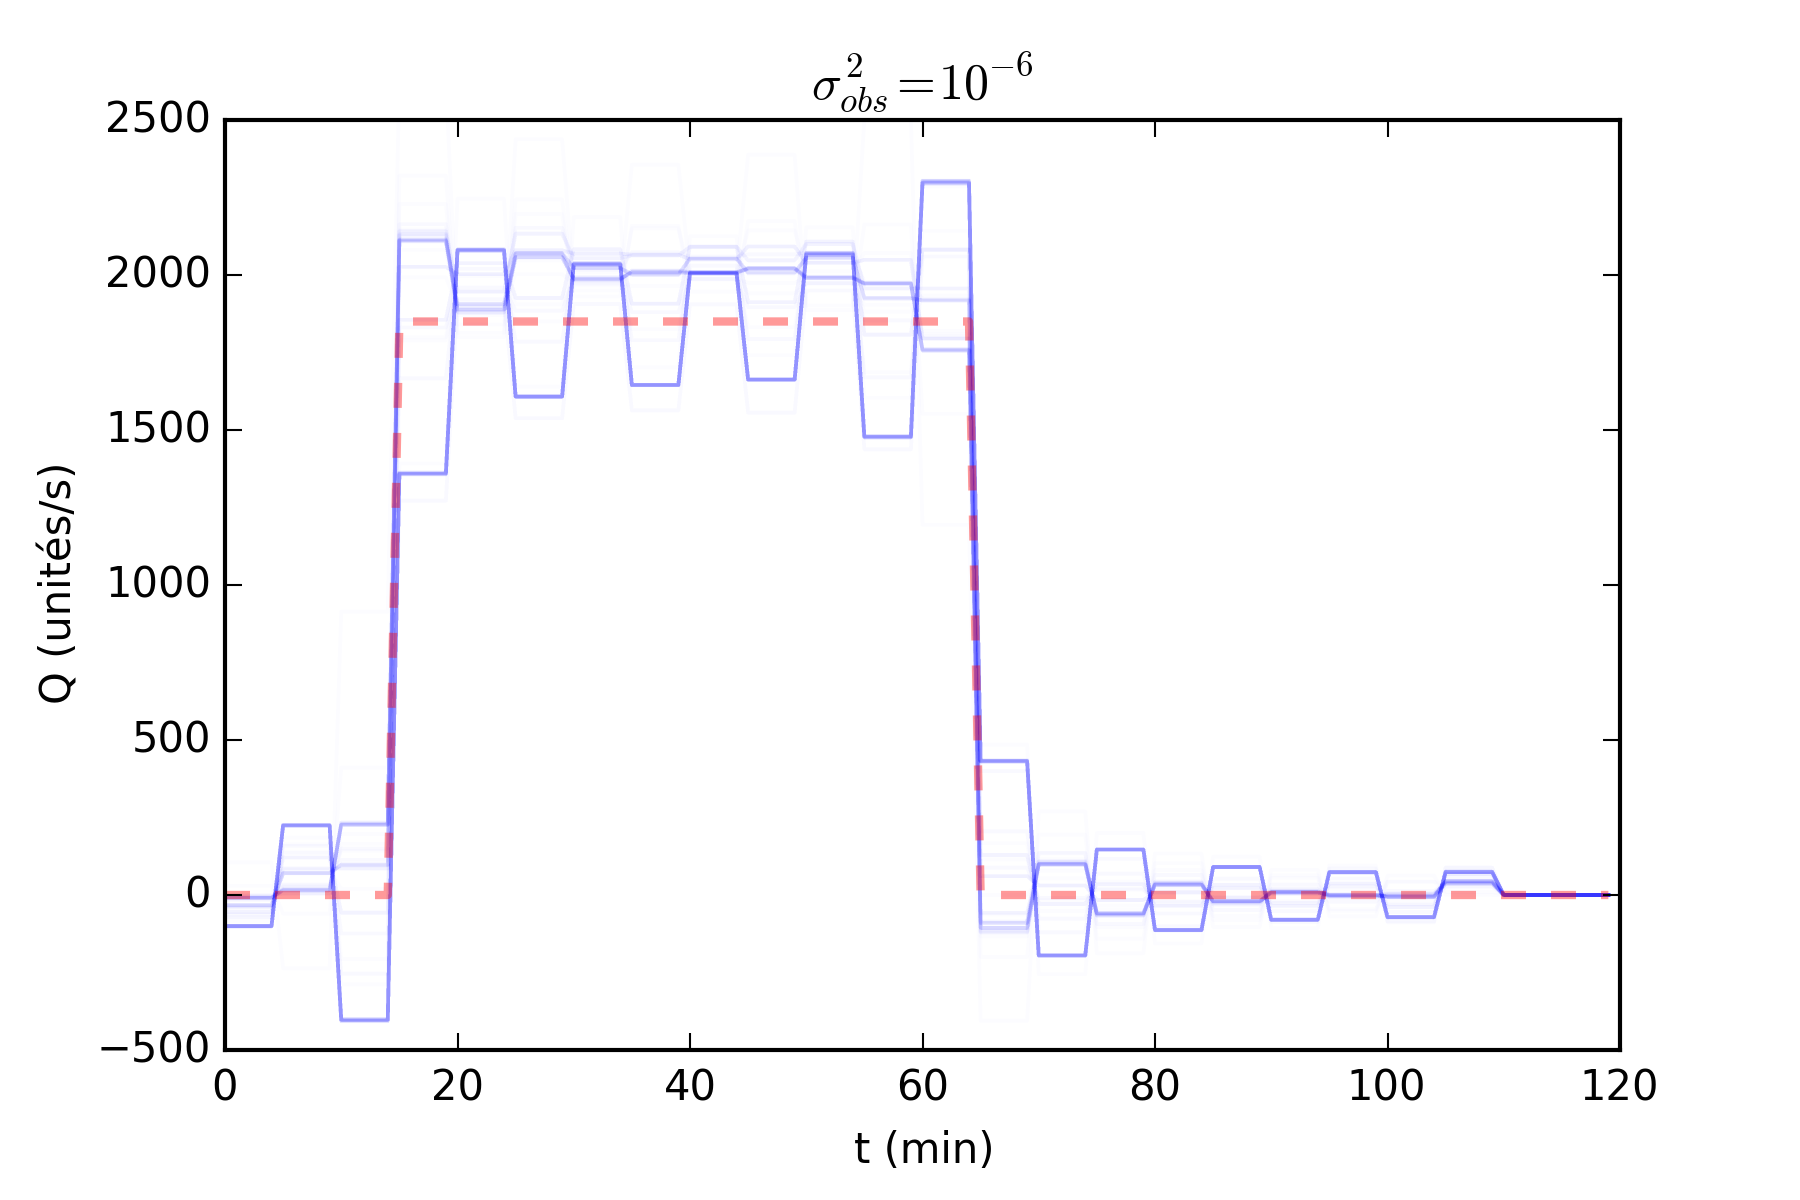
\includegraphics[width=1\textwidth]{25C_varobs_Q_C.png}
  		\caption{}
  		\label{varC_q}
  	\end{subfigure}%
  	\begin{subfigure}[t]{0.5\textwidth}
  		\centering
  		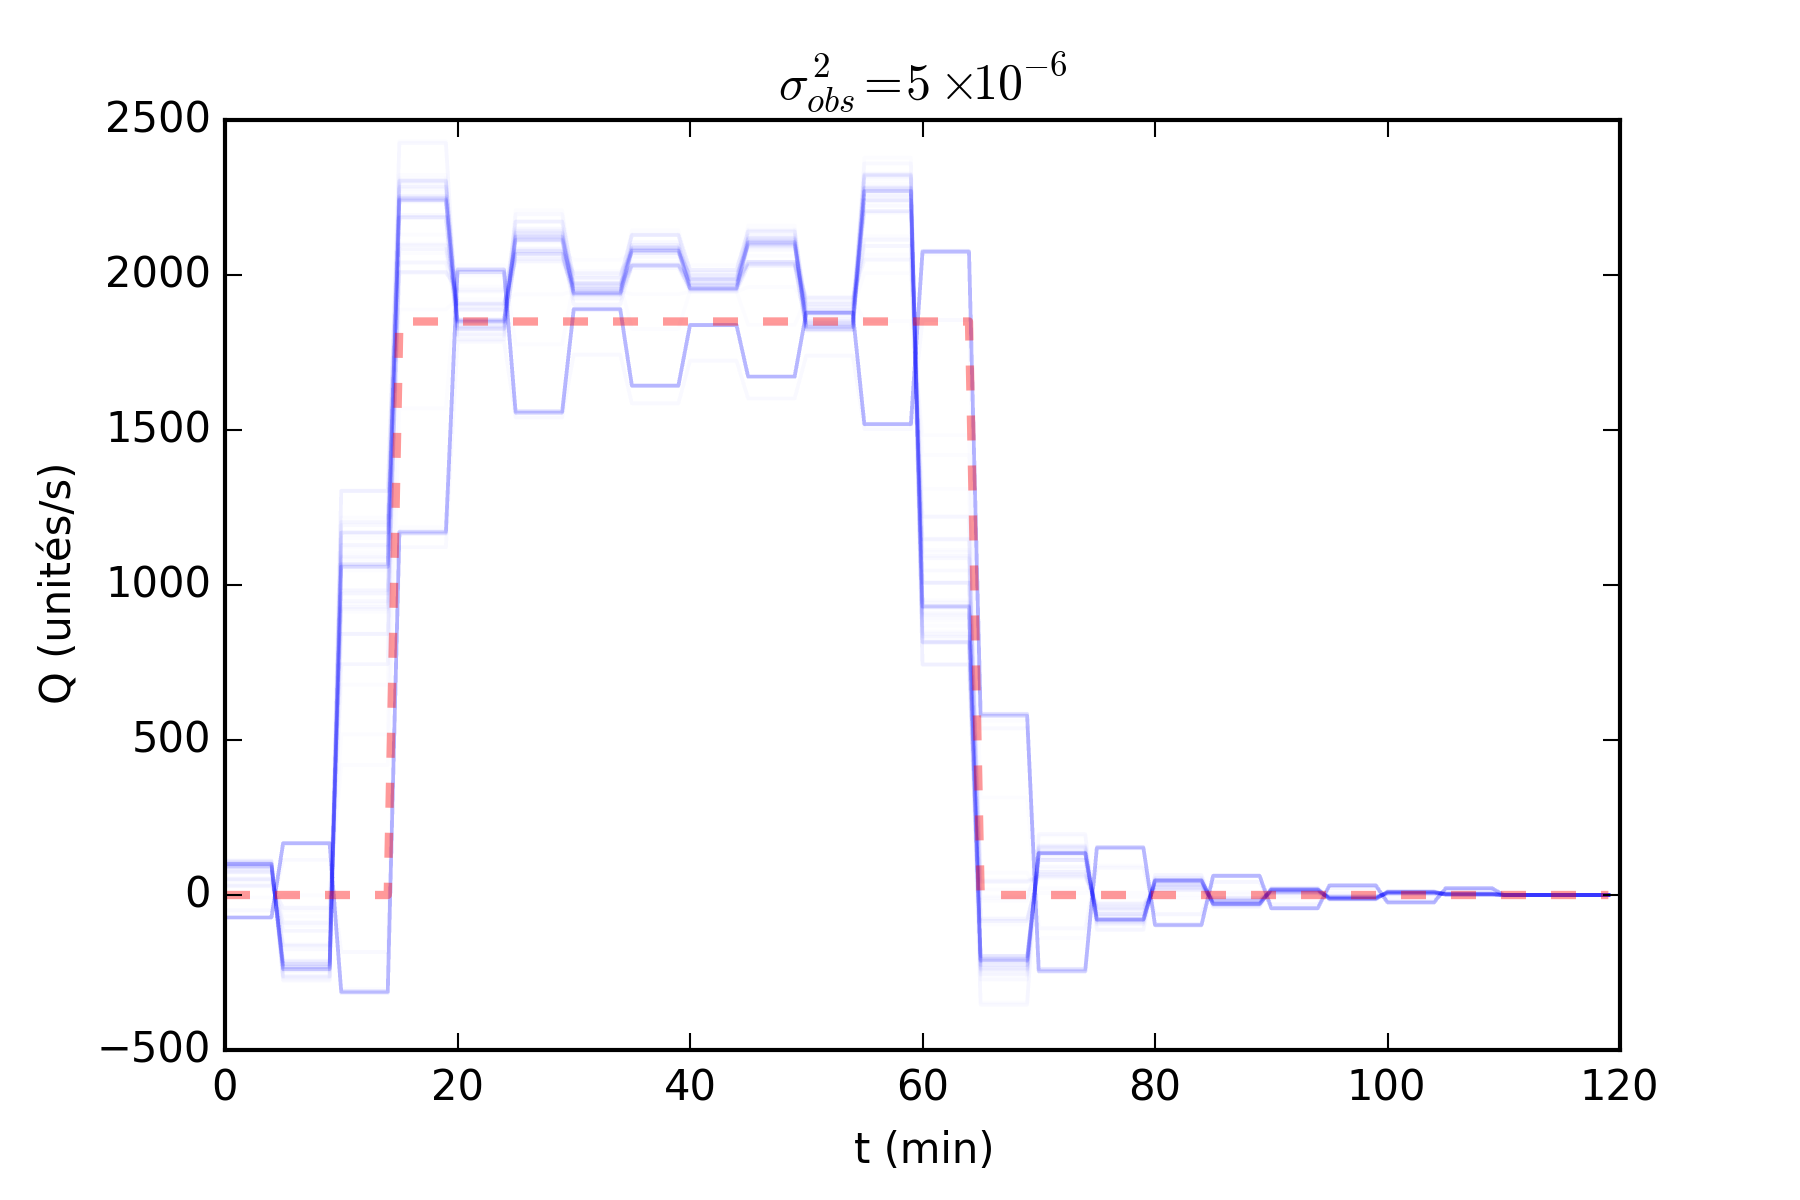
\includegraphics[width=1\textwidth]{25C_varobs_Q_D.png}
  		\caption{}
  		\label{varD_q}
  	\end{subfigure}
  	\begin{subfigure}[t]{0.5\textwidth}
  		\centering
  		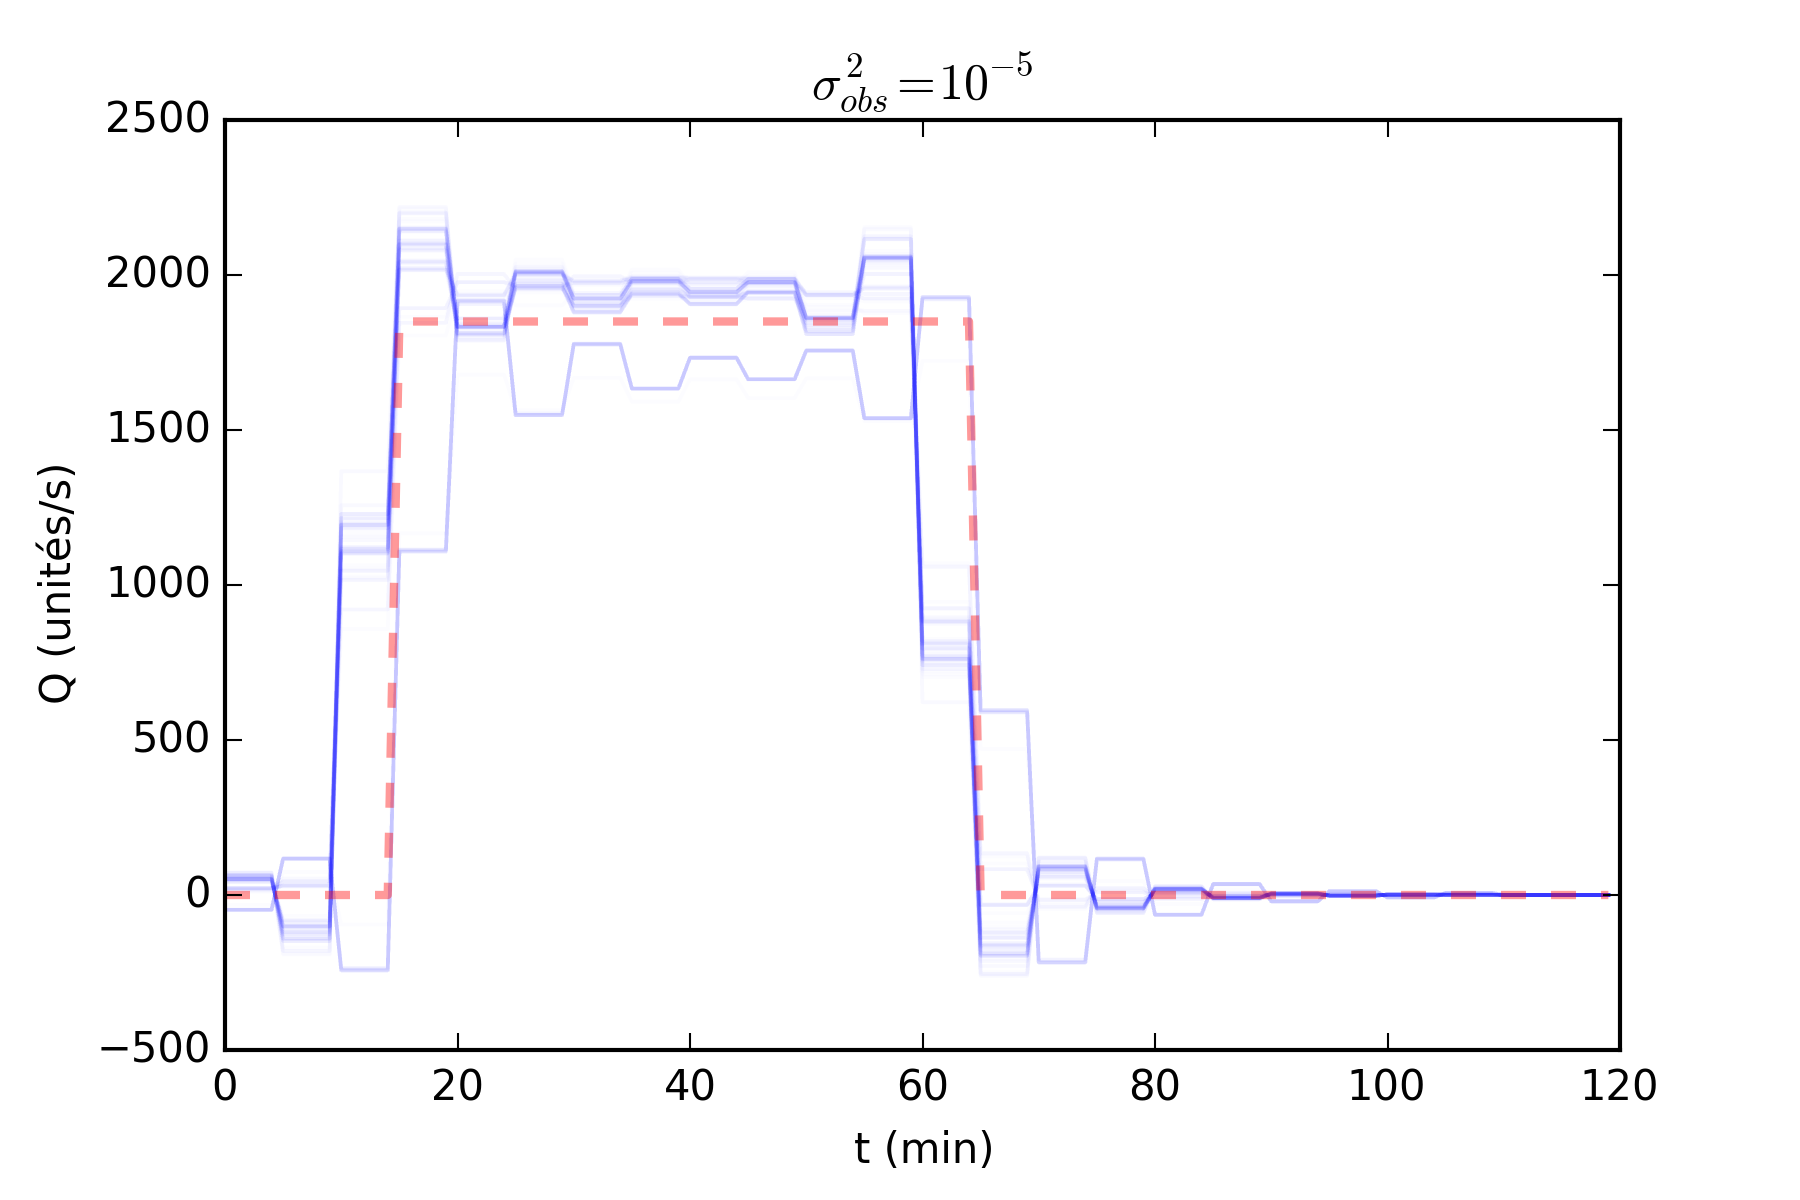
\includegraphics[width=1\textwidth]{25C_varobs_Q_E.png}
  		\caption{}
  		\label{varE_q}
  	\end{subfigure}%
  	\begin{subfigure}[t]{0.5\textwidth}
  		\centering
  		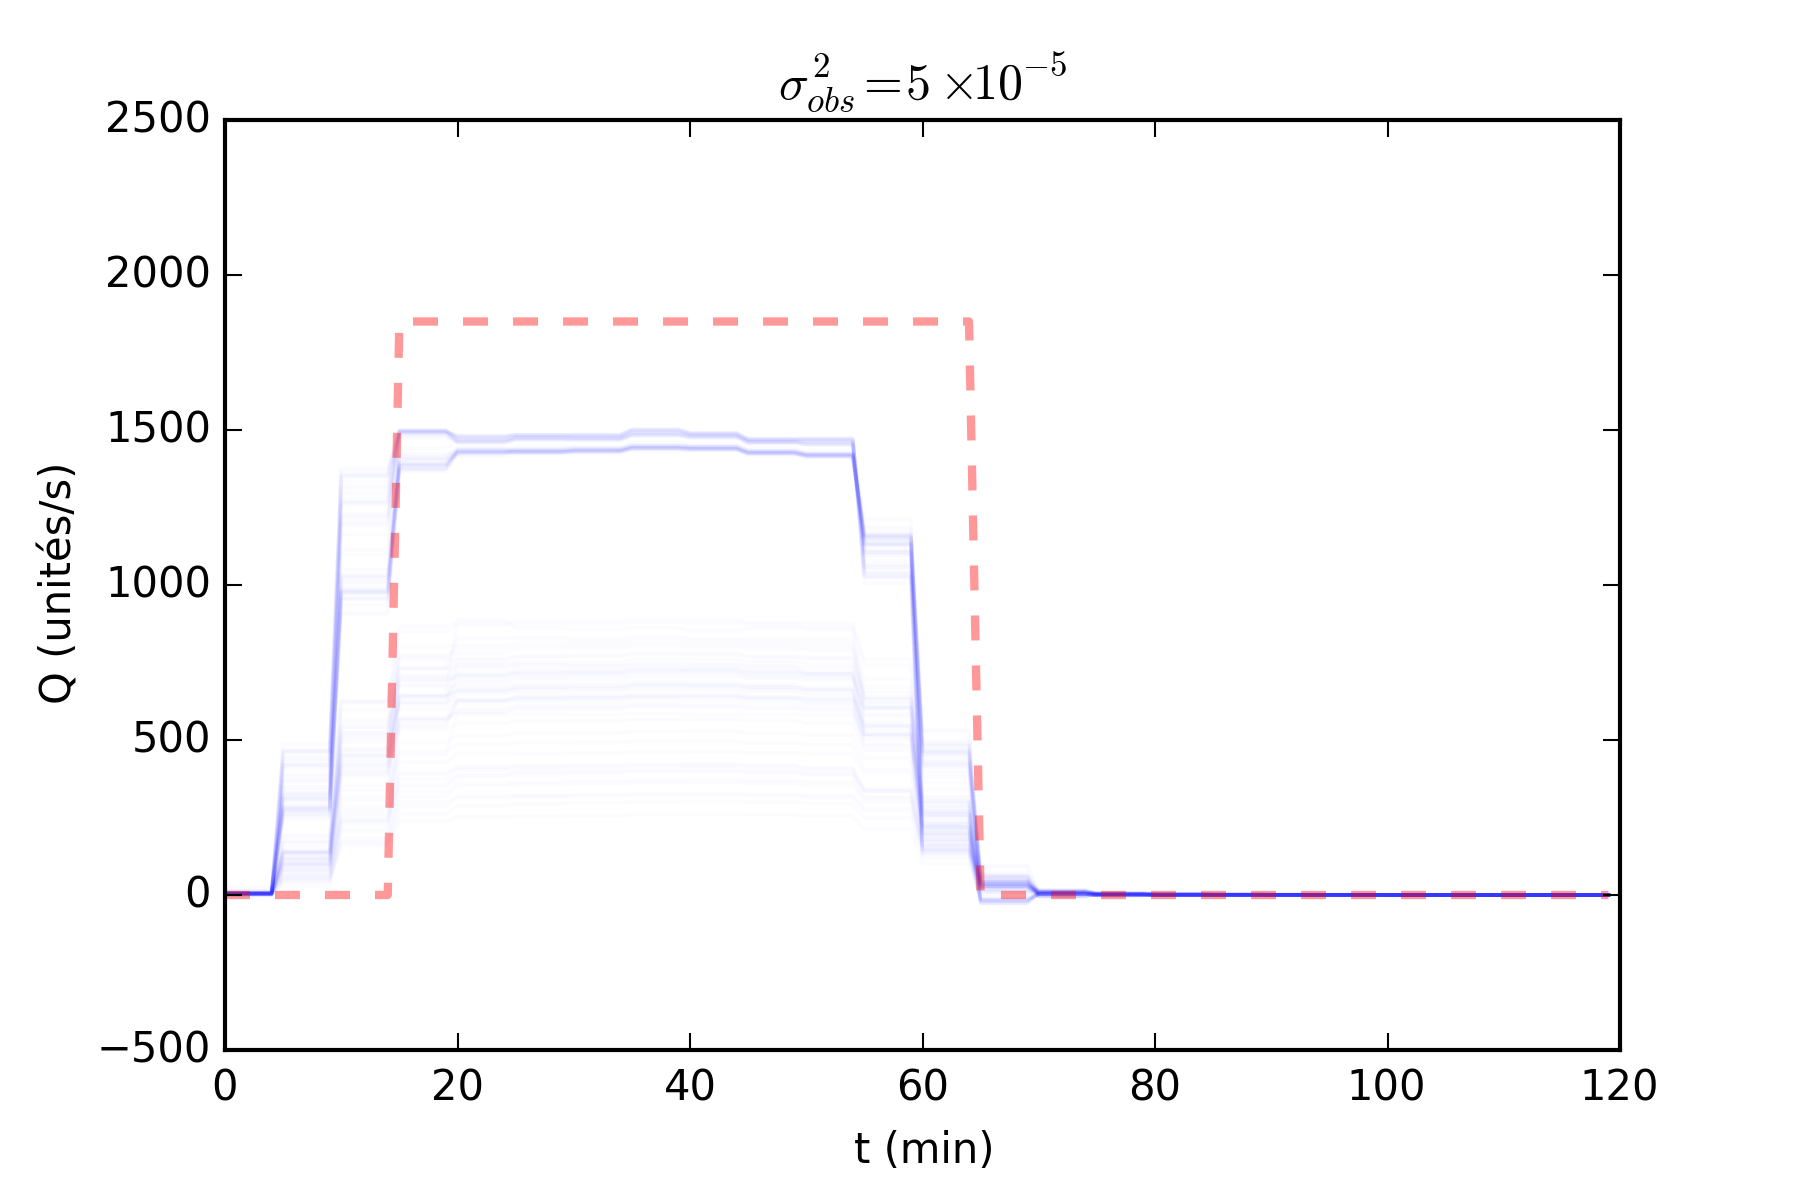
\includegraphics[width=1\textwidth]{25C_varobs_Q_F.png}
  		\caption{}
  		\label{varF_q}
  	\end{subfigure}
  	\caption{Analyse paramétrique sur la variance d'observation $\varObs$ pour le cas-test Beaune (25 capteurs): reconstruction du profil d'émission}
  	\label{fig_25C_analyse_varobs_q}
  \end{figure}
  
    \begin{figure}[p!]
    	\centering
    	\begin{subfigure}[t]{0.5\textwidth}
    		\centering
    		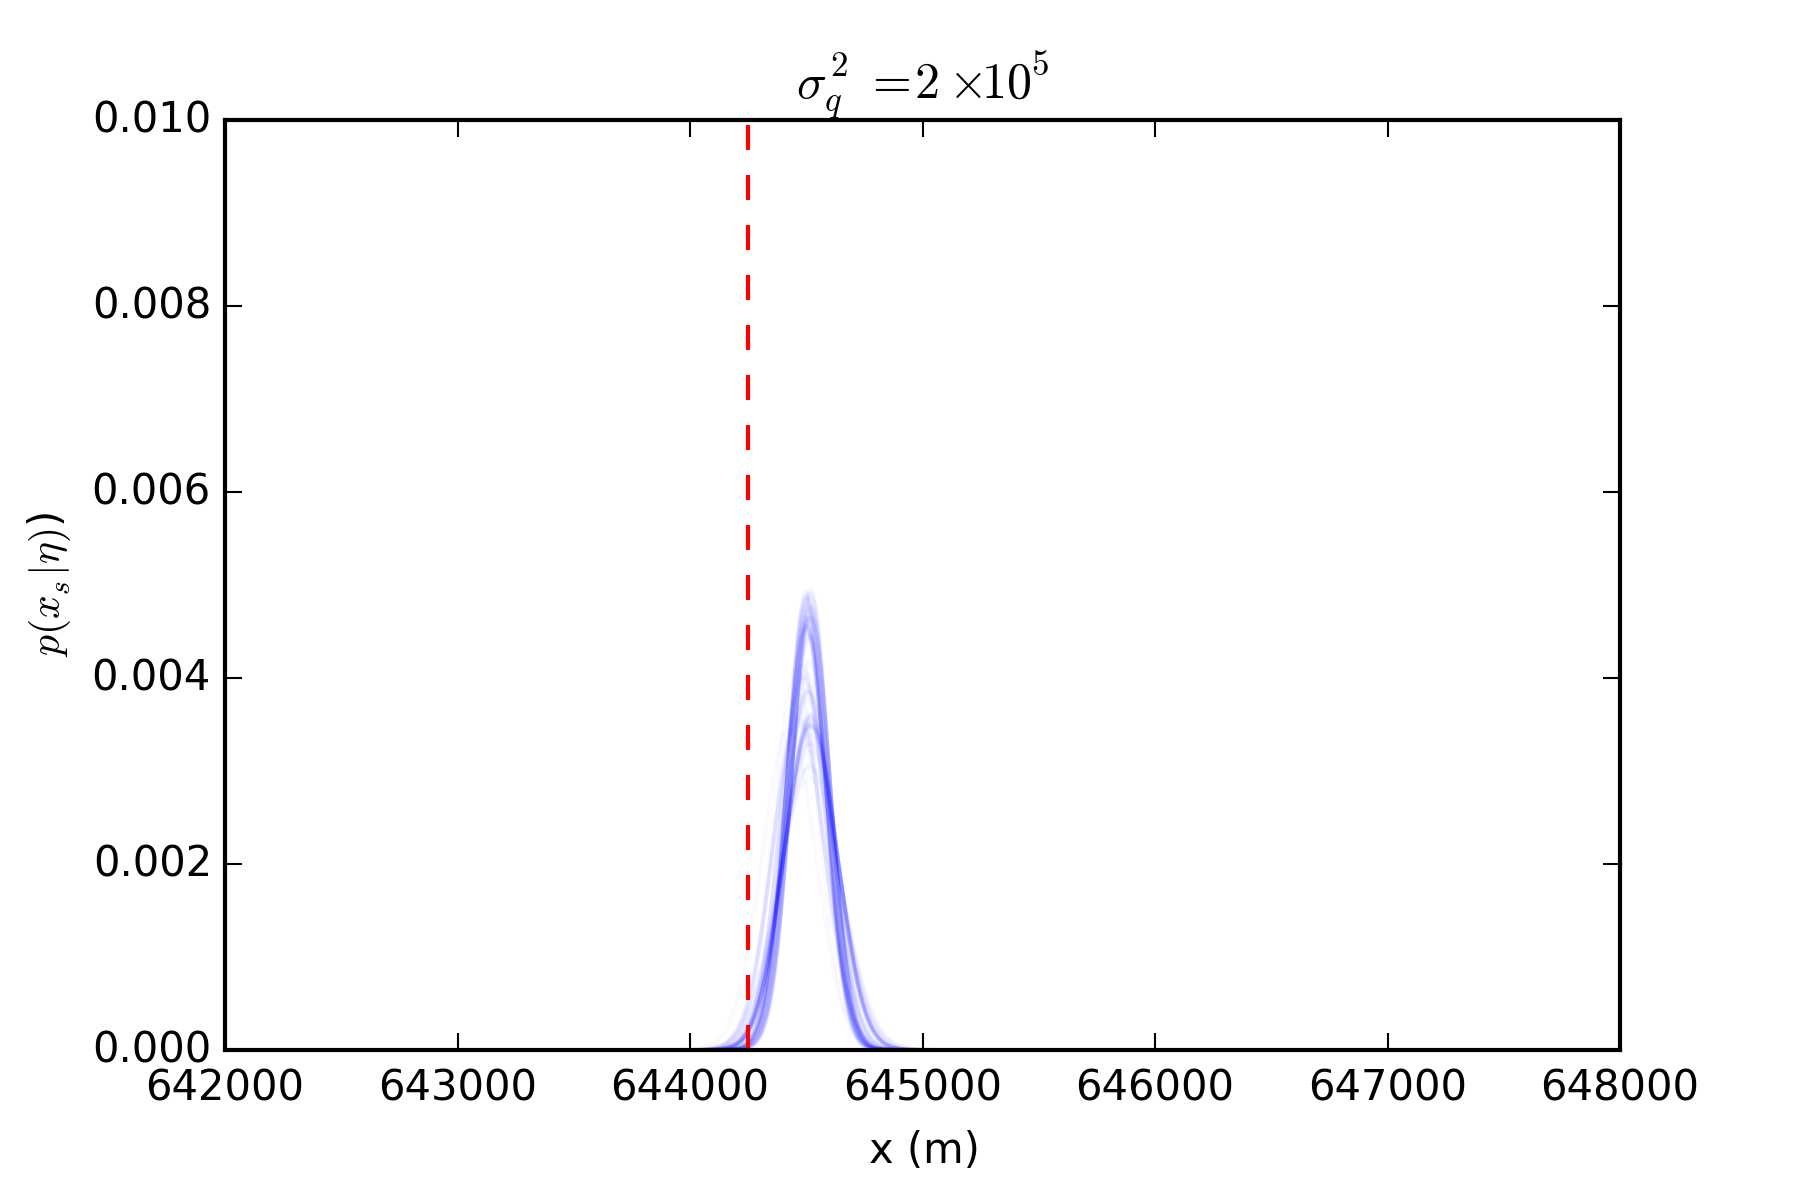
\includegraphics[width=1\textwidth]{25C_varq_X_A.png}
    		\caption{}
    		\label{varq_A_x}
    	\end{subfigure}%
    	\begin{subfigure}[t]{0.5\textwidth}
    		\centering
    		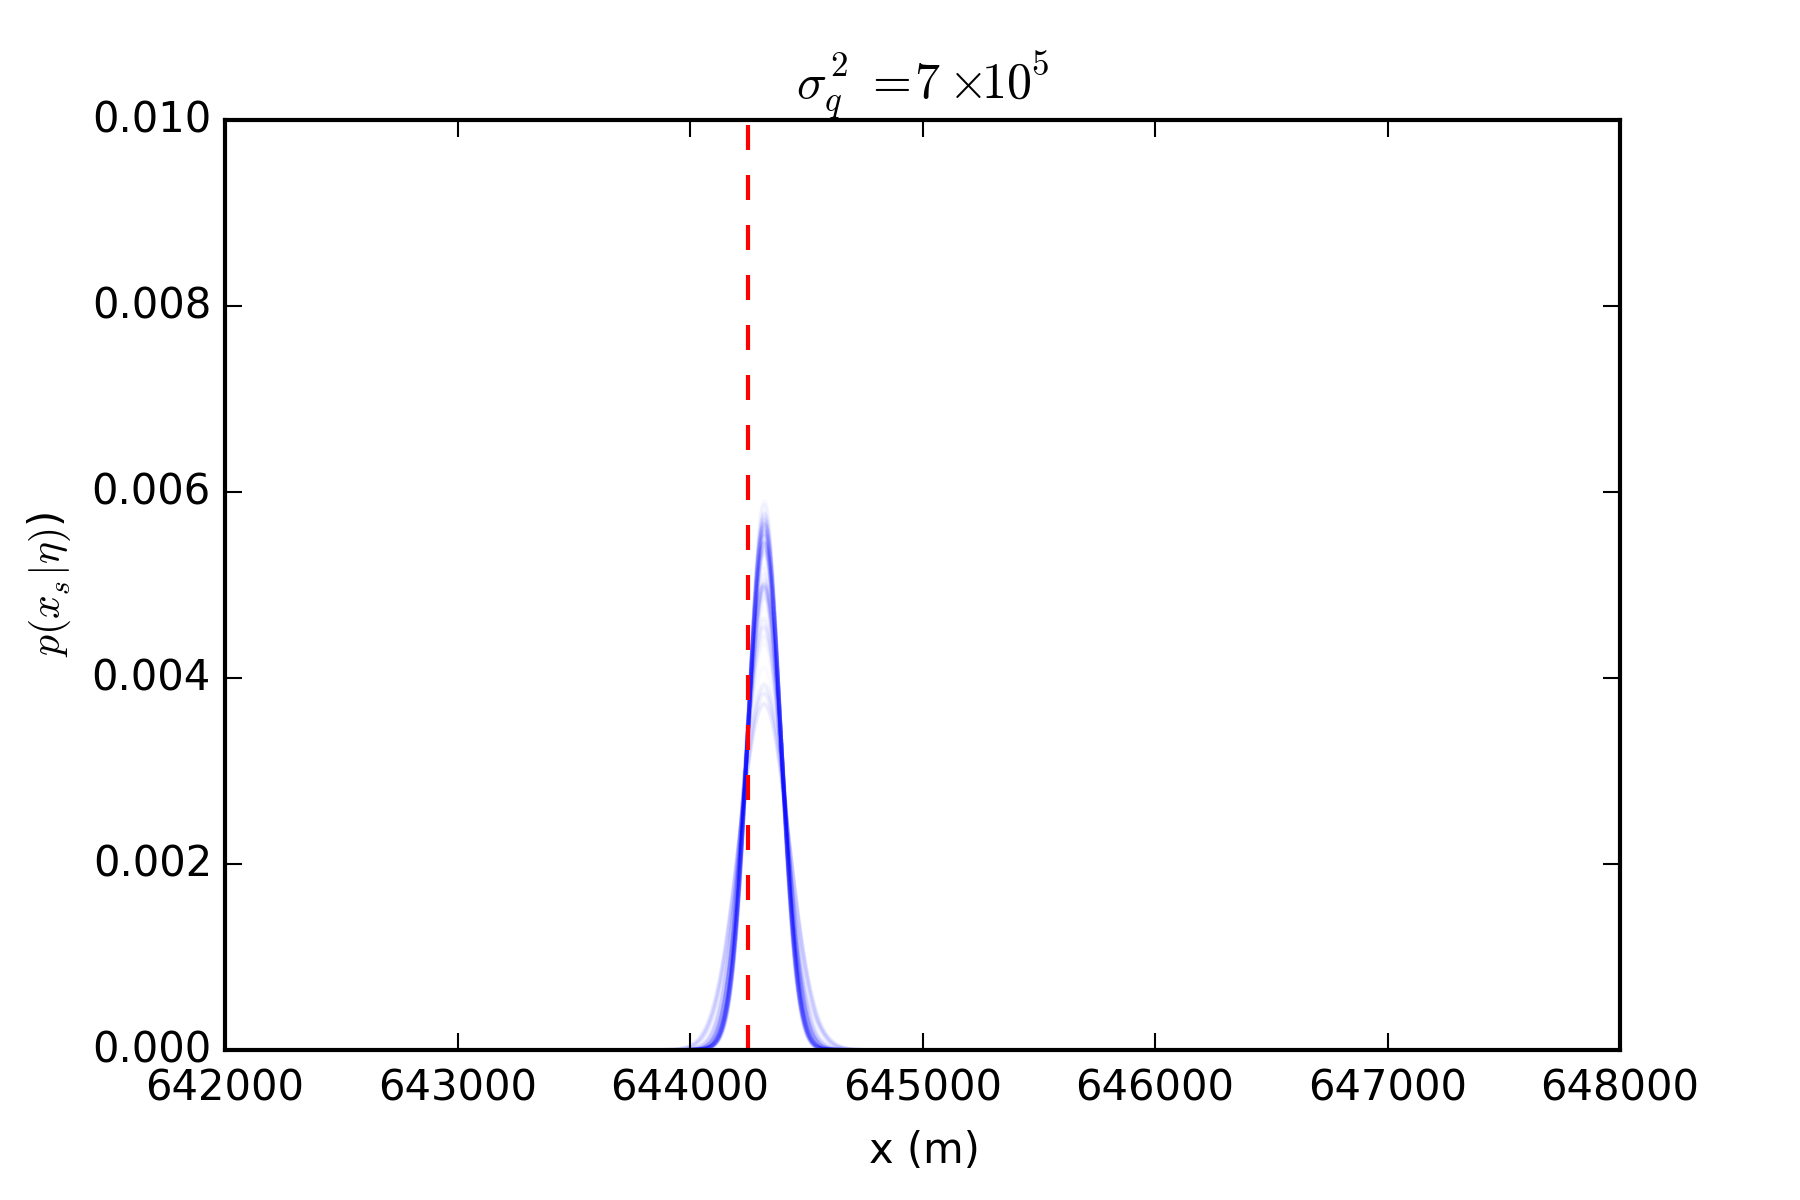
\includegraphics[width=1\textwidth]{25C_varq_X_B.png}
    		\caption{}
    		\label{varq_B_x}
    	\end{subfigure}
    	\begin{subfigure}[t]{0.5\textwidth}
    		\centering
    		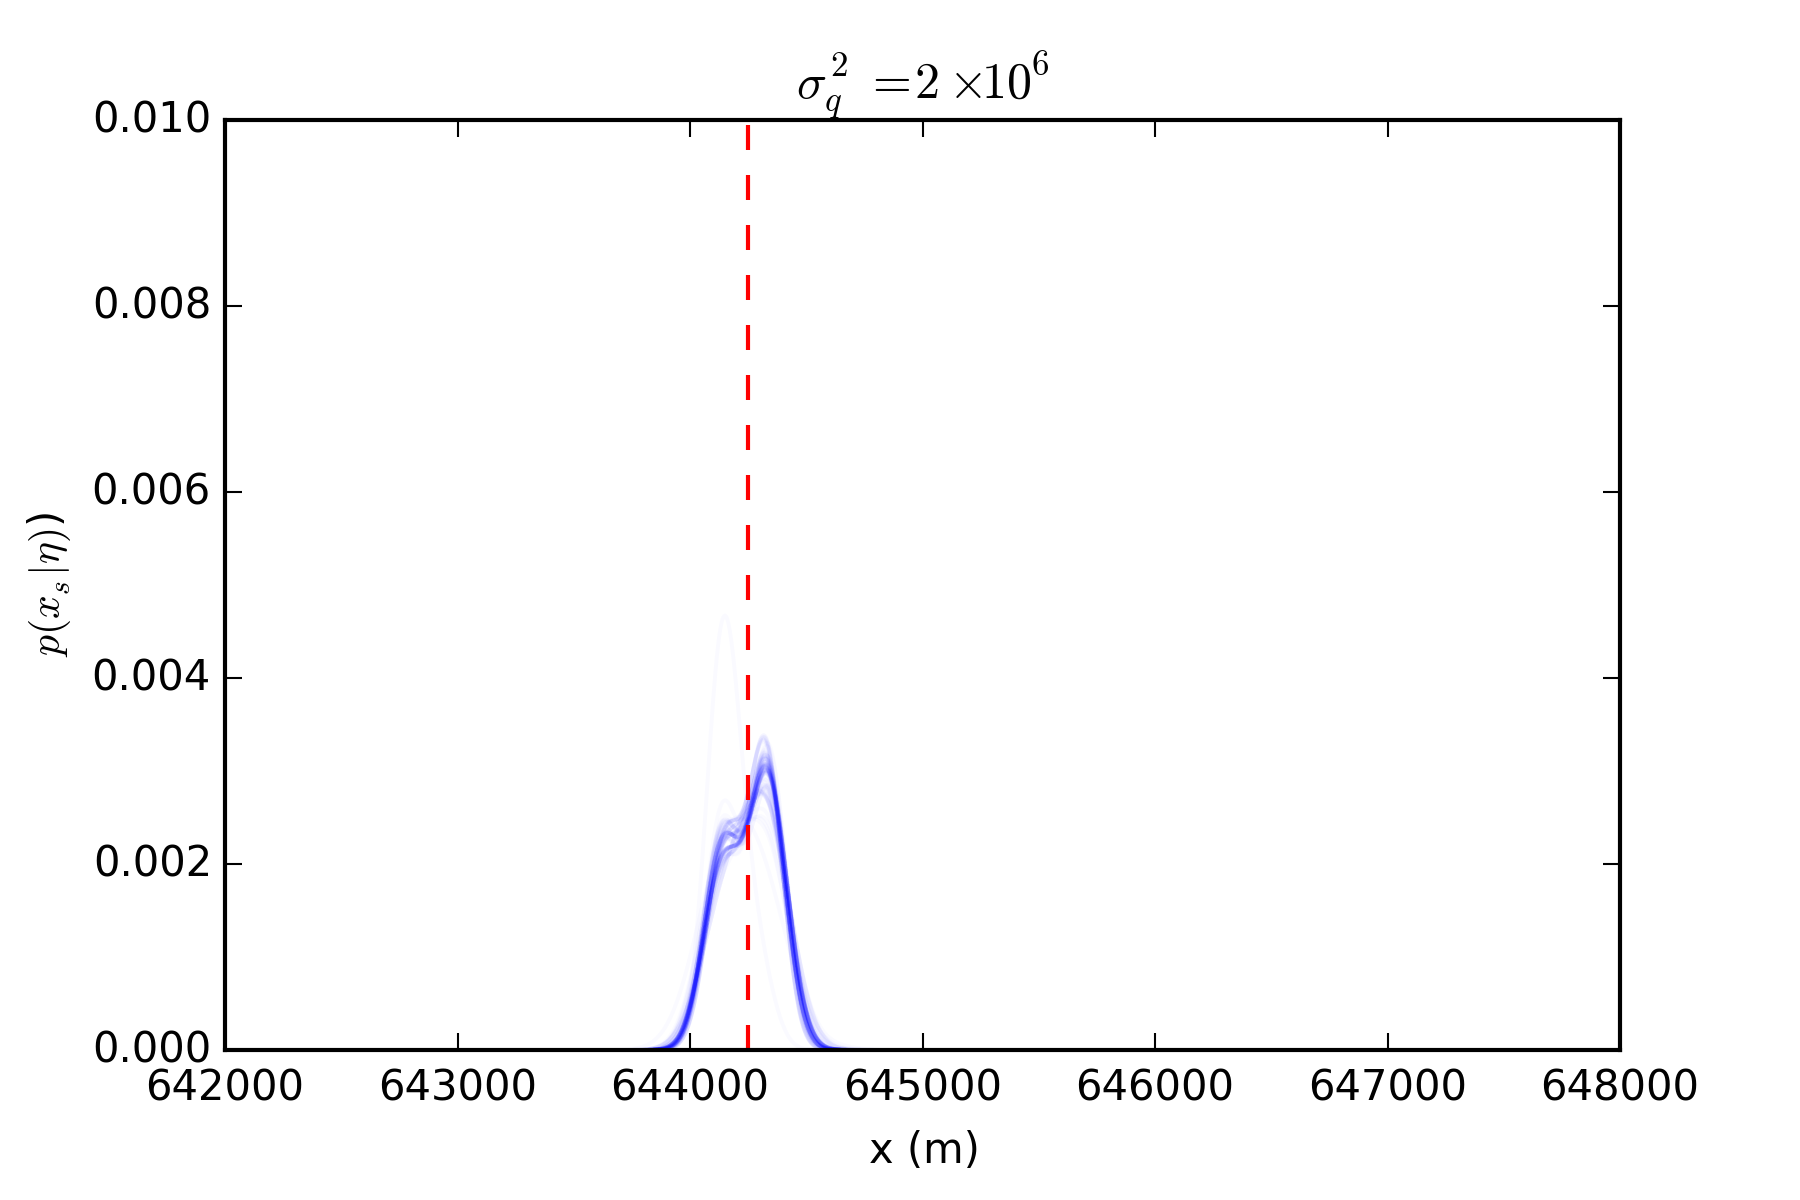
\includegraphics[width=1\textwidth]{25C_varq_X_C.png}
    		\caption{}
    		\label{varq_C_x}
    	\end{subfigure}%
    	\begin{subfigure}[t]{0.5\textwidth}
    		\centering
    		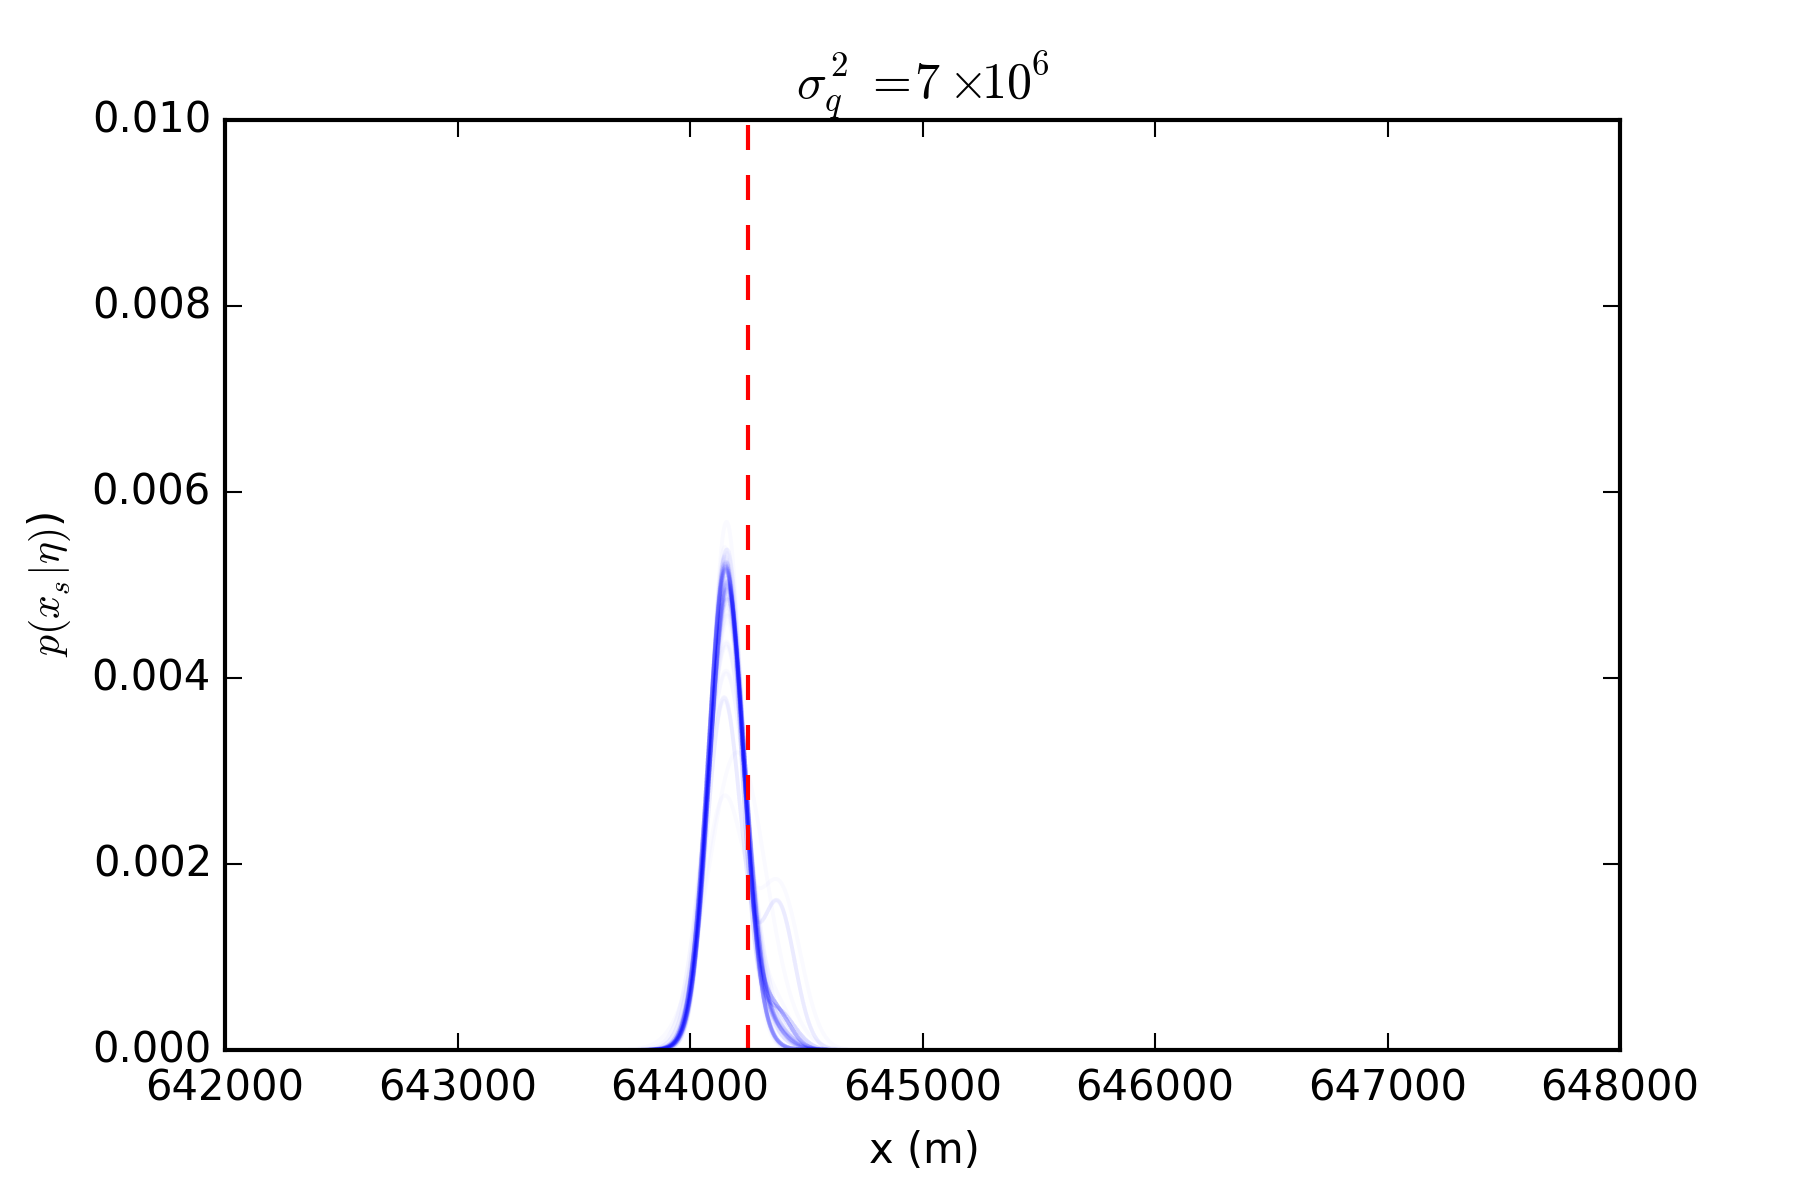
\includegraphics[width=1\textwidth]{25C_varq_X_D.png}
    		\caption{}
    		\label{varq_D_x}
    	\end{subfigure}
    	\begin{subfigure}[t]{0.5\textwidth}
    		\centering
    		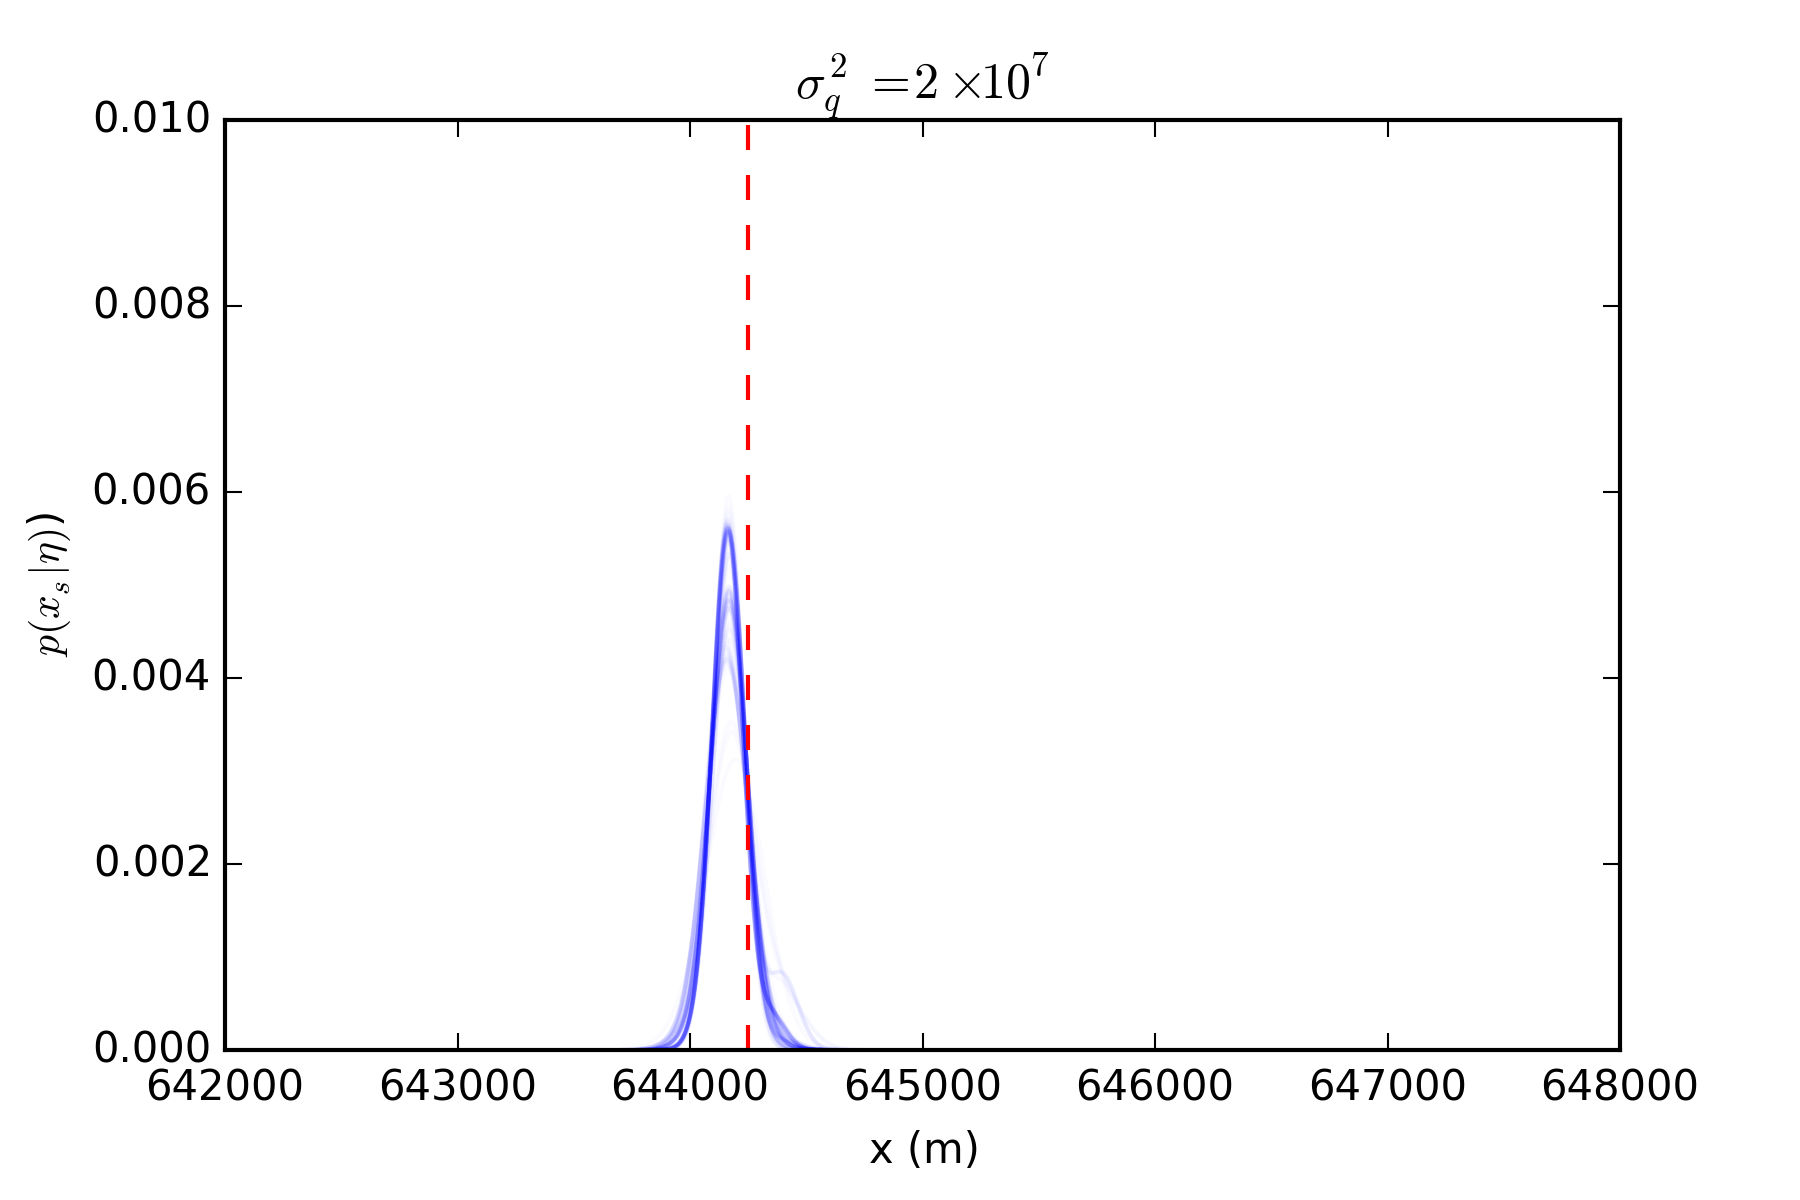
\includegraphics[width=1\textwidth]{25C_varq_X_E.png}
    		\caption{}
    		\label{varq_E_x}
    	\end{subfigure}%
    	\begin{subfigure}[t]{0.5\textwidth}
    		\centering
    		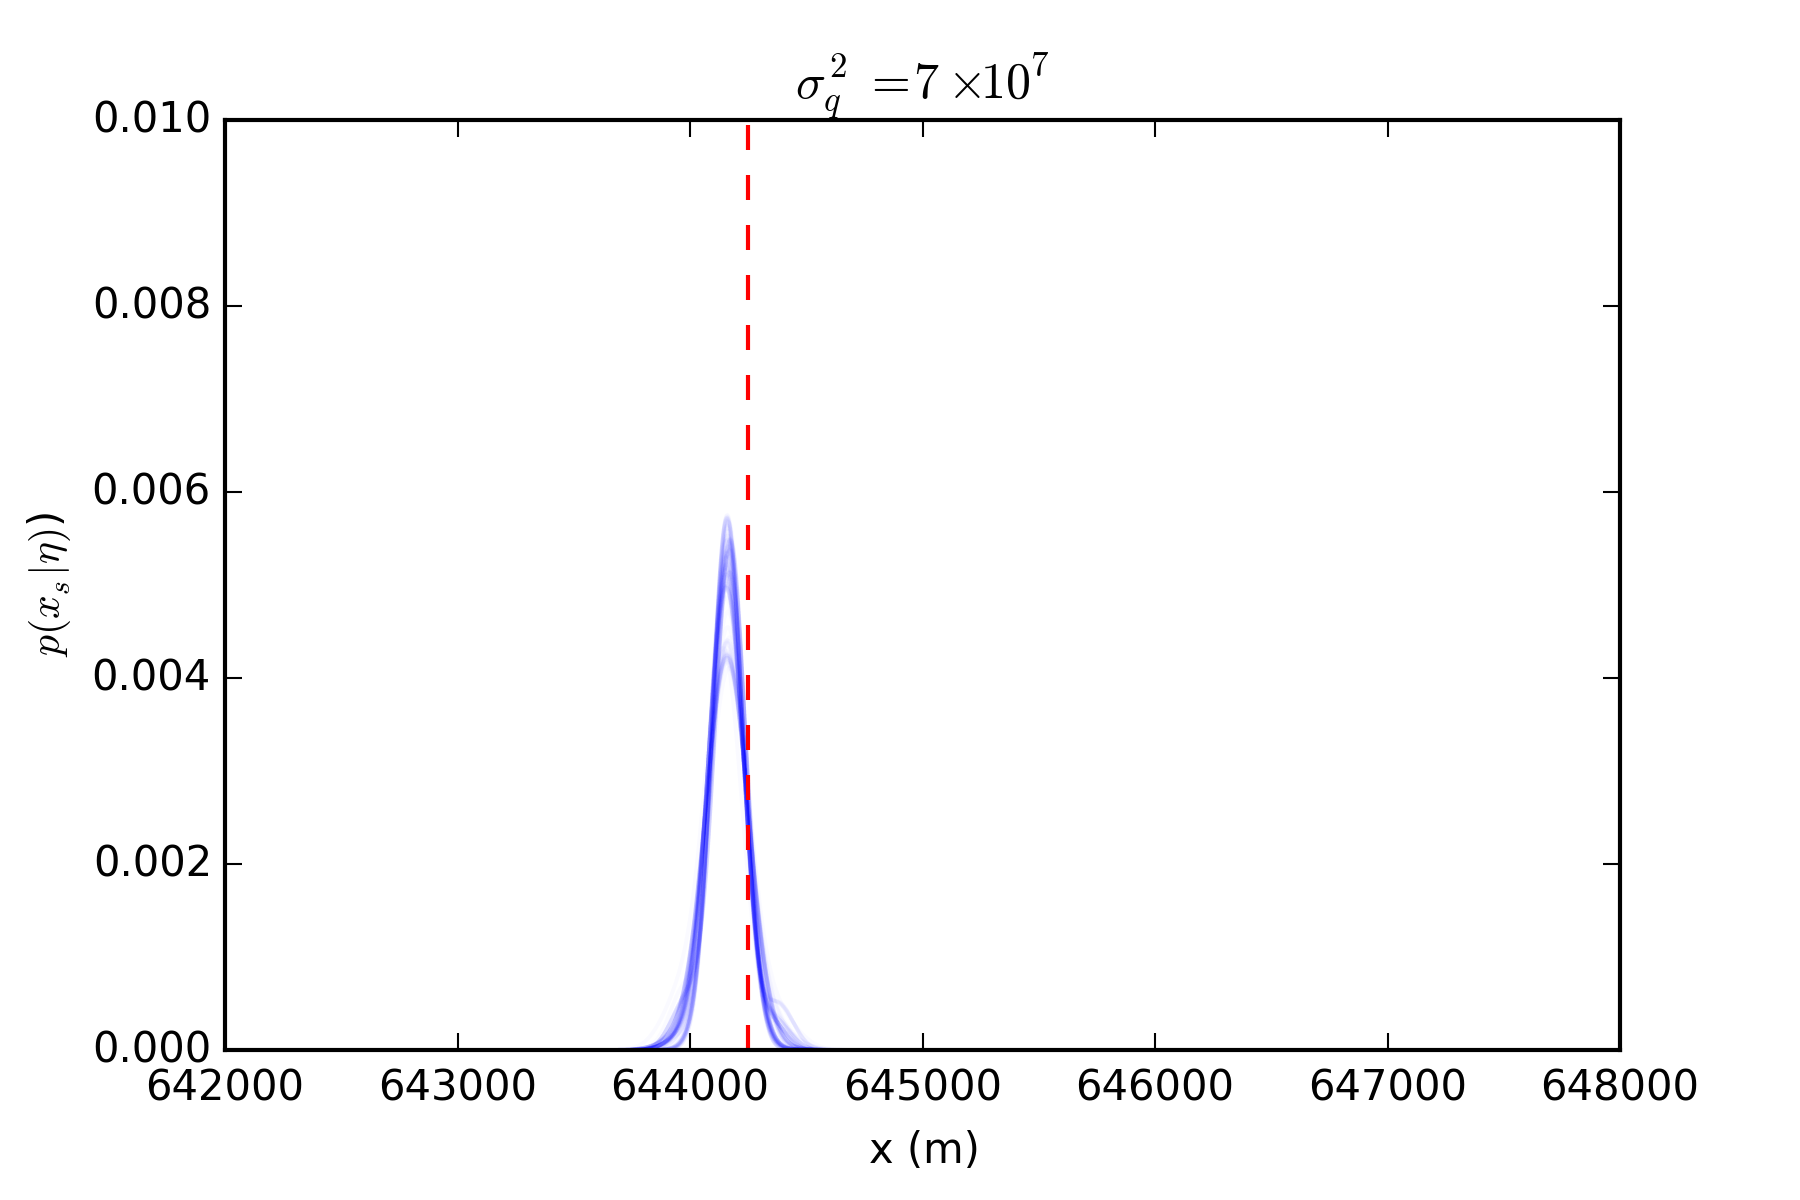
\includegraphics[width=1\textwidth]{25C_varq_X_F.png}
    		\caption{}
    		\label{varq_F_x}
    	\end{subfigure}
    	\caption{Analyse paramétrique sur la variance a priori $\varQ$ pour le cas-test Beaune (25 capteurs): localisation en $x$ de la source}
    	\label{fig_25C_analyse_varq_x}
    \end{figure}
    
    \begin{figure}[p!]
    	\centering
    	\begin{subfigure}[t]{0.5\textwidth}
    		\centering
    		\includegraphics[width=1\textwidth]{25C_varq_Y_A.png}
    		\caption{}
    		\label{varq_A_y}
    	\end{subfigure}%
    	\begin{subfigure}[t]{0.5\textwidth}
    		\centering
    		\includegraphics[width=1\textwidth]{25C_varq_Y_B.png}
    		\caption{}
    		\label{varq_B_y}
    	\end{subfigure}
    	\begin{subfigure}[t]{0.5\textwidth}
    		\centering
    		\includegraphics[width=1\textwidth]{25C_varq_Y_C.png}
    		\caption{}
    		\label{varq_C_y}
    	\end{subfigure}%
    	\begin{subfigure}[t]{0.5\textwidth}
    		\centering
    		\includegraphics[width=1\textwidth]{25C_varq_Y_D.png}
    		\caption{}
    		\label{varq_D_y}
    	\end{subfigure}
    	\begin{subfigure}[t]{0.5\textwidth}
    		\centering
    		\includegraphics[width=1\textwidth]{25C_varq_Y_E.png}
    		\caption{}
    		\label{varq_E_y}
    	\end{subfigure}%
    	\begin{subfigure}[t]{0.5\textwidth}
    		\centering
    		\includegraphics[width=1\textwidth]{25C_varq_Y_F.png}
    		\caption{}
    		\label{varq_F_y}
    	\end{subfigure}
    	\caption{Analyse paramétrique sur la variance a priori $\varQ$ pour le cas-test Beaune (25 capteurs): localisation en $y$ de la source}
    	\label{fig_25C_analyse_varq_y}
    \end{figure}
    
    \begin{figure}[p!]
    	\centering
    	\begin{subfigure}[t]{0.5\textwidth}
    		\centering
    		\includegraphics[width=1\textwidth]{25C_varq_Q_A.png}
    		\caption{}
    		\label{varq_A_q}
    	\end{subfigure}%
    	\begin{subfigure}[t]{0.5\textwidth}
    		\centering
    		\includegraphics[width=1\textwidth]{25C_varq_Q_B.png}
    		\caption{}
    		\label{varq_B_q}
    	\end{subfigure}
    	\begin{subfigure}[t]{0.5\textwidth}
    		\centering
    		\includegraphics[width=1\textwidth]{25C_varq_Q_C.png}
    		\caption{}
    		\label{varq_C_q}
    	\end{subfigure}%
    	\begin{subfigure}[t]{0.5\textwidth}
    		\centering
    		\includegraphics[width=1\textwidth]{25C_varq_Q_D.png}
    		\caption{}
    		\label{varq_D_q}
    	\end{subfigure}
    	\begin{subfigure}[t]{0.5\textwidth}
    		\centering
    		\includegraphics[width=1\textwidth]{25C_varq_Q_E.png}
    		\caption{}
    		\label{varq_E_q}
    	\end{subfigure}%
    	\begin{subfigure}[t]{0.5\textwidth}
    		\centering
    		\includegraphics[width=1\textwidth]{25C_varq_Q_F.png}
    		\caption{}
    		\label{varq_F_q}
    	\end{subfigure}
    	\caption{Analyse paramétrique sur la variance a priori $\varQ$ pour le cas-test Beaune (25 capteurs): reconstruction du profil d'émission}
    	\label{fig_25C_analyse_varq_q}
    \end{figure}